\documentclass[11pt]{article}

\usepackage[a4paper,margin=1in]{geometry}
\usepackage[T1]{fontenc}
\usepackage[utf8]{inputenc}
\usepackage{lmodern}
\usepackage{microtype}
\usepackage{amsmath,amssymb,amsthm,mathtools}
\usepackage{xcolor}
\usepackage{bm}
\usepackage{booktabs}
\usepackage{array}
\usepackage{enumitem}
\usepackage{graphicx}
\usepackage{hyperref}
\usepackage[nameinlink,noabbrev]{cleveref}

\hypersetup{
  colorlinks=true,
  linkcolor=blue,
  citecolor=blue,
  urlcolor=blue
}

\definecolor{deepnavy}{HTML}{0D1B2A}
\definecolor{signalblue}{HTML}{1D4ED8}
\definecolor{tealgreen}{HTML}{0F766E}
\definecolor{warmgold}{HTML}{C77D12}
\definecolor{stressred}{HTML}{B42318}

\newtheorem{theorem}{Theorem}[section]
\newtheorem{corollary}[theorem]{Corollary}
\newtheorem{definition}[theorem]{Definition}
\newtheorem{remark}[theorem]{Remark}
\newtheorem{proposition}[theorem]{Proposition}
\newtheorem{lemma}[theorem]{Lemma}

\newcommand{\R}{\mathbb{R}}
\newcommand{\E}{\mathbb{E}}
\newcommand{\cT}{\mathcal{T}}
\newcommand{\Shat}{\widehat{S}}
\newcommand{\Ghat}{\widehat{G}}
\newcommand{\tr}{\operatorname{tr}}
\newcommand{\Var}{\operatorname{Var}}
\newcommand{\TV}{\operatorname{TV}}
\newcommand{\RePart}{\operatorname{Re}}
\newcommand{\ImPart}{\operatorname{Im}}
\newcommand{\dd}{\,\mathrm{d}}
\newcommand{\REV}{}

\title{A Conditional Fluctuation--Dissipation Identity for Market Impact:\\
Diagnostics, Reconstruction, and an Order-Book Pilot}
\author{Atharva Parande\\MIT ADT University\\Computer Science}
\date{April 2026}

\begin{document}

\maketitle

\begin{abstract}
\REV
In physical systems at equilibrium, the response to an external perturbation is tied to the system's own fluctuations through the fluctuation--dissipation theorem (FDT). This paper asks whether an analogous relation can be formulated for transient market impact. We work with Stieltjes propagator kernels, namely completely monotone impact kernels that are compatible with no-dynamic-arbitrage in linear impact models, and study the conditional implications of an explicit latent modal equilibrium model. Under that model one obtains the frequency-domain identity
\[
  \ImPart \Ghat(i\omega)=\frac{\omega}{2\Theta}S_P(\omega),
\]
where $\Ghat$ is the Fourier--Laplace transform of the impact kernel, $S_P$ is the price power spectral density, and $\Theta$ is a scalar market thermal index. The value of the identity is empirical as much as theoretical: it yields a falsifiable equilibrium restriction, a structured inverse problem for the hidden relaxation measure, and a market-state map built from thermal intensity and equilibrium deviation. The paper develops a linear-Gaussian Kyle--OU foundation, a converse characterization in second-order law, a uniqueness result for $\Theta$ on nondegenerate frequency bands, an explicit testing procedure, and a constrained spectral reconstruction program. Monte Carlo experiments show correct size and rising power. Real-data evidence based on public LOBSTER order-book samples for June 21, 2012 finds that AAPL is broadly FDT-consistent at the open and close but rejected at midday with $p=0.003$, while the inferred thermal index moves from $4.07$ to $1.17$ and then back to $2.22$. A same-date cross-section across AAPL, GOOG, and AMZN shows that this midday breakdown is not mechanically present in every liquid name, which supports the interpretation of the diagnostic as a market-state filter rather than a tautological intraday pattern.
\end{abstract}

\section{Introduction and Motivation}

\subsection{Why a Frequency-Domain View}
Market impact and volatility are usually estimated in separate empirical workflows. The impact kernel is inferred from order flow and returns, while price spectra are studied as a property of returns alone. The central question of this paper is whether those two objects are governed by the same hidden relaxation geometry. A frequency-domain formulation is attractive because it places response and fluctuation on the same observable scale and turns equilibrium into a directly testable spectral restriction. The analogy is with the fluctuation--dissipation theorem of statistical physics: not because markets are literal thermal systems, but because admissible transient-impact models share the same passive-systems structure.

\subsection{Core Hypothesis}
The main identity proposed in this manuscript is
\begin{equation}\label{eq:main-fdt}
  \ImPart \Ghat(i\omega)=\frac{\omega}{2\Theta}S_P(\omega),
  \qquad \text{for a.e.\ }\omega>0.
\end{equation}
Here $\Theta$ is a market thermal index: large values indicate abundant noise-trader activity relative to permanent impact, while small values indicate a colder and potentially more fragile market.
The paper does not claim to derive this identity from a fully general strategic equilibrium model. Instead, it formulates a latent modal equilibrium model under which the identity must hold and then asks whether that restriction is empirically useful and empirically falsifiable.

\begin{remark}[Why the conditional framing is still powerful]
The central empirical content of the paper lies in rejection as much as in confirmation. If the FDT restriction fails on a frequency band of positive measure, then the observed market cannot belong to the latent modal equilibrium class studied here. In that sense the paper should be read as a falsification framework for an economically structured model class, not merely as an attempt to confirm one specific mechanism.
\end{remark}

\subsection{Contributions}
\REV
The paper makes five concrete contributions:
\begin{enumerate}[label=\arabic*.]
  \item A latent-modal equilibrium framework for transient impact together with a linear-Gaussian Kyle--OU foundation that explains why Stieltjes kernels and the thermal normalization arise naturally in a zero-profit filtering economy.
  \item A conditional fluctuation--dissipation identity and a converse characterization, yielding an equivalence in second-order law between the FDT restriction and a latent modal representation.
  \item A testing theory for the thermal index and the deviation functional, including a median-of-ratios estimator, a null distribution, and a null-enforcing bootstrap.
  \item A constrained inverse problem for recovering the latent relaxation spectrum, together with matrix-valued extensions of the identity, test statistic, and reconstruction step.
  \item An empirical layer consisting of Monte Carlo evidence, rolling synthetic validation, and real-data LOBSTER evidence with a same-date three-name cross-section.
\end{enumerate}

\subsection{Related Literature}
\REV
This paper sits at the intersection of admissible transient-impact theory, spectral inference for high-frequency data, and locally stationary time-series methods. On the structural side, Rosenbaum and Tomas~\cite{RosenbaumTomas2022} study admissibility restrictions for transient cross-impact models and thereby clarify which kernels rule out dynamic-arbitrage pathologies. The present manuscript stays inside the Stieltjes subclass of that admissible world and asks a complementary question: once an admissible transient kernel is posited, what observable frequency-domain restriction must hold if the market is also governed by the latent modal equilibrium model introduced below?

\REV
For rolling-window inference, the appropriate asymptotic backdrop is the locally stationary framework of Dahlhaus~\cite{Dahlhaus1997,Dahlhaus1996}, because the empirical sections allow thermal conditions and deviation profiles to evolve across the day even when each local window is treated as approximately stationary.

The paper proceeds in three steps. \Cref{sec:equilibrium,sec:fdt} introduce the latent modal equilibrium class and the conditional FDT identity it implies. \Cref{sec:testing,sec:inverse} convert that identity into an estimable diagnostic and, when the null is not rejected, an inverse problem for the hidden relaxation spectrum. \Cref{sec:monte-carlo,sec:rolling,sec:lobster-pilot,sec:roadmap} then show what the diagnostic looks like in synthetic data and in a focused real-data order-book study.

\begin{figure}[t]
\centering
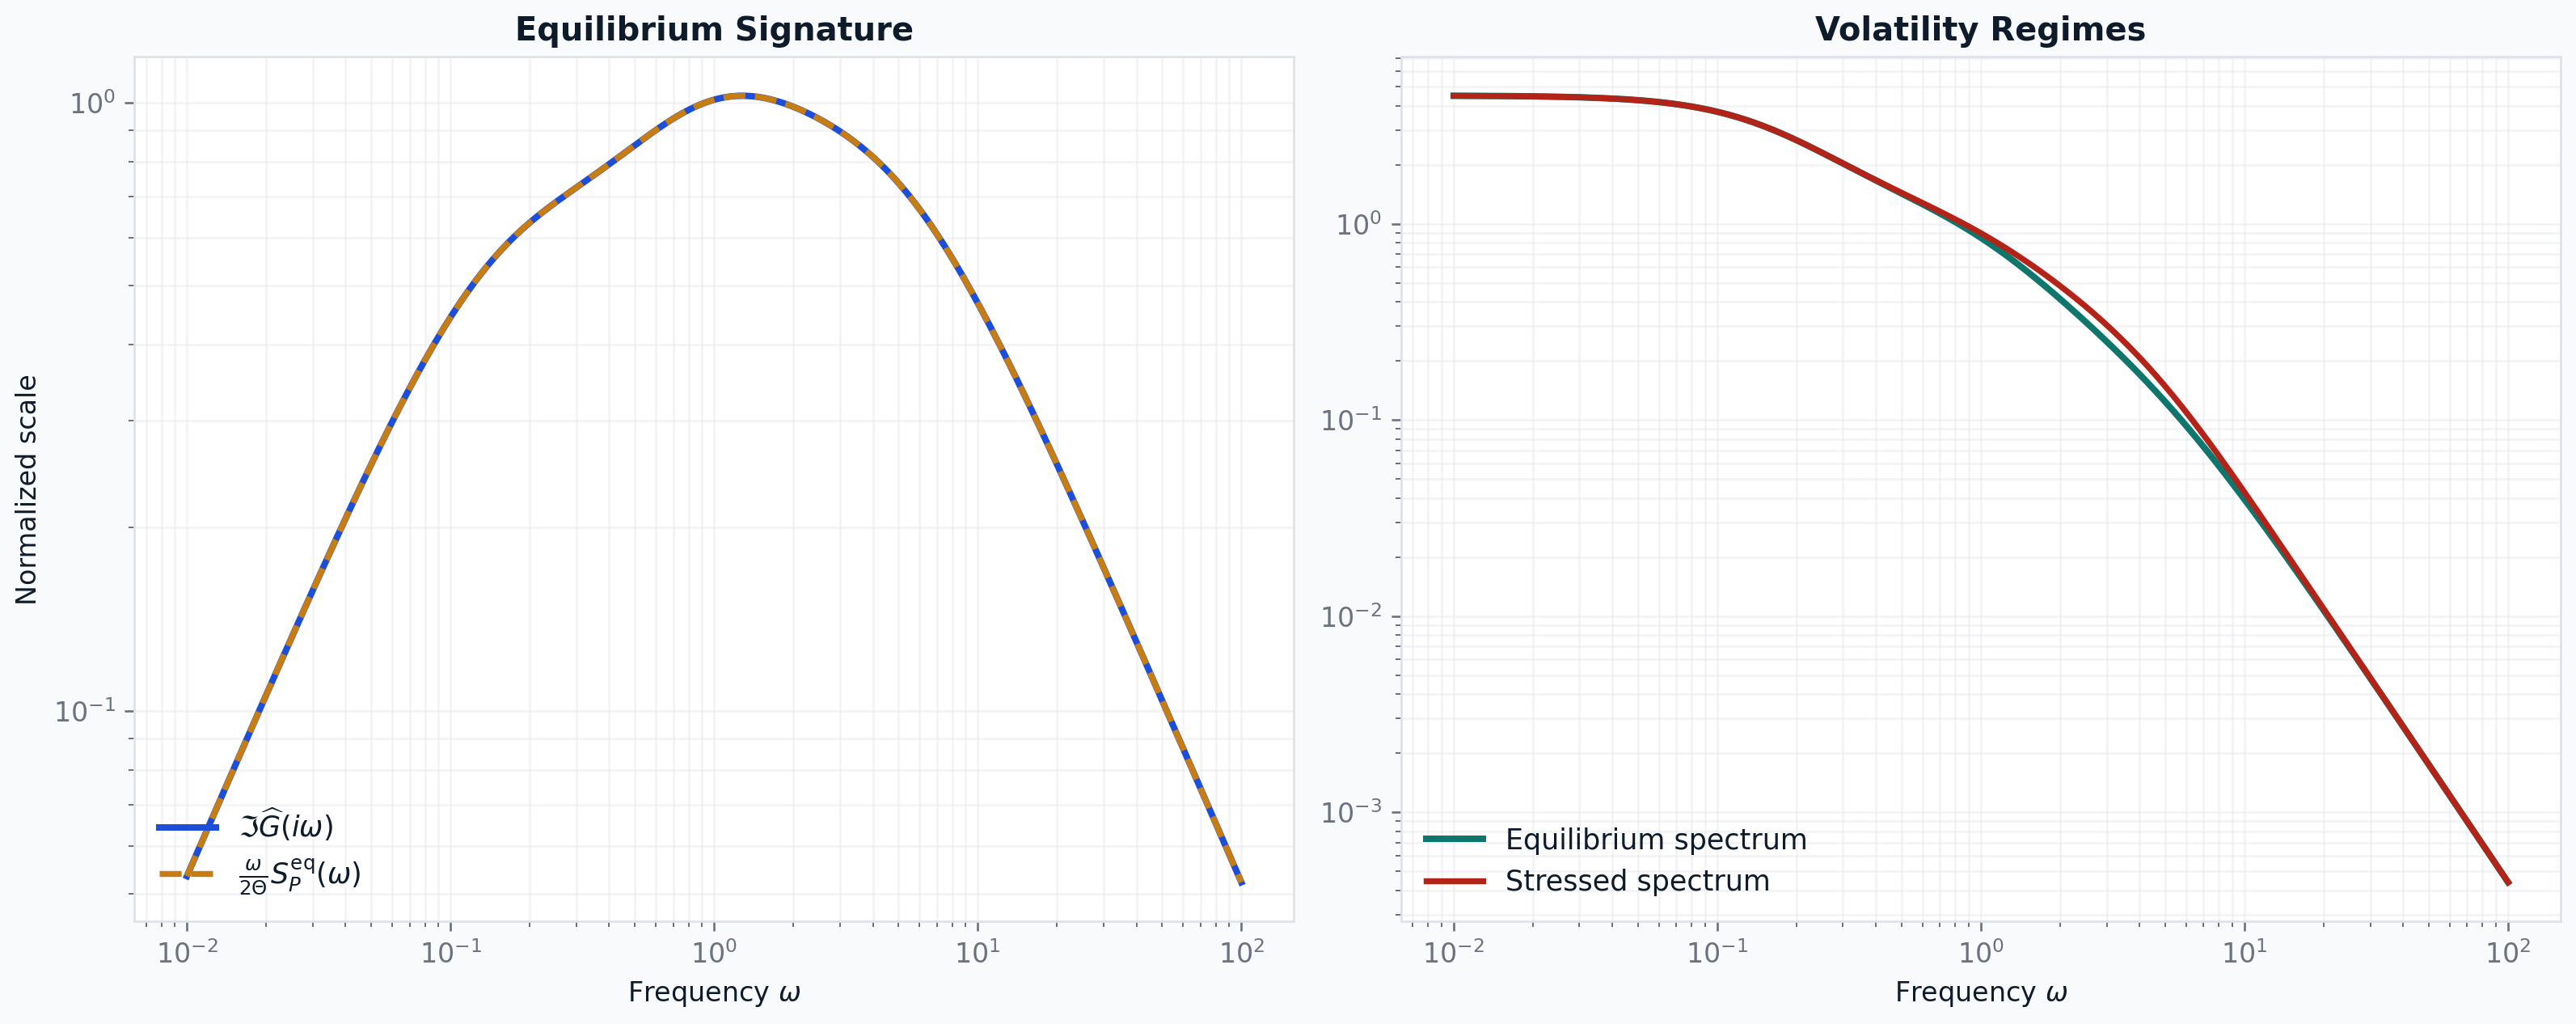
\includegraphics[width=\textwidth]{figures/generated/fdt_signature.png}
\caption{Conceptual signature of the proposed market FDT. In the left panel, the blue curve is $\Im \Ghat(i\omega)$ and the dashed gold curve is $(\omega/(2\Theta))S_P^{\mathrm{eq}}(\omega)$; they overlap under equilibrium. In the right panel, the teal equilibrium spectrum is contrasted with a red stressed spectrum that generates a nonzero deviation functional $\Delta(\omega)$.}
\label{fig:fdt-signature}
\end{figure}

\section{Mathematical Setup and Assumptions}\label{sec:setup}

\subsection{Price Formation Model}
Consider an agent trading $d$ assets over a horizon $[0,T]$. Let $u(t)\in\R^d$ denote the trading rate and define cumulative order flow
\[
  Q(t)=\int_0^t u(s)\dd s.
\]
The observed price process is modeled as
\begin{equation}\label{eq:price-model}
  P(t)=\int_{-\infty}^t G(t-s)\,\dd Q(s)+L(t), \qquad t\in[0,T],
\end{equation}
where $G:\R_+\to\mathbb{S}^d$ is a causal impact kernel and $L(t)$ is a square-integrable martingale representing public-information innovations, orthogonal to order flow.

\subsection{Stieltjes Propagators}
\begin{definition}[Stieltjes propagator]
The kernel $G$ is a \emph{Stieltjes propagator} if it admits the representation
\begin{equation}\label{eq:stieltjes-time}
  G(t)=g_\infty \delta(t)+\int_{(0,\infty)} e^{-\rho t} M(\dd \rho), \qquad t>0,
\end{equation}
where $g_\infty\in\mathbb{S}_+^d$ and $M$ is a positive $\mathbb{S}_+^d$-valued Borel measure on $(0,\infty)$ satisfying
\[
  \int_0^\infty \frac{\rho}{1+\rho}\,|M|(\dd\rho)<\infty.
\]
\end{definition}

Its Fourier--Laplace transform is
\begin{equation}\label{eq:laplace-transform}
  \Ghat(z)=g_\infty + \int_0^\infty \frac{\rho}{\rho+z} M(\dd\rho), \qquad \RePart z>0.
\end{equation}

Representative examples are:
\begin{enumerate}[label=\arabic*.]
  \item Single exponential: $G(t)=A e^{-\rho_0 t}$.
  \item Finite mixture: $G(t)=\sum_{k=1}^r A_k e^{-\rho_k t}$.
  \item Power law: $G(t)=Ct^{-\alpha}$ for $\alpha\in(0,1)$, represented by a continuous relaxation measure.
\end{enumerate}

\subsection{Core Structural Assumptions}
\REV
We use the following structural assumptions throughout the equilibrium and FDT sections:
\begin{enumerate}[label=\textbf{A\arabic*}.]
  \item $G$ is a Stieltjes propagator with $g_\infty\succeq 0$ and positive relaxation measure $M$.
  \item Price follows \cref{eq:price-model}.
  \item $L(t)$ is a square-integrable martingale orthogonal to order flow.
  \item $\Ghat(i\omega)\neq 0$ on the retained frequency band.
  \item Either $g_\infty\succ 0$ or $M$ has no atom at $\rho=0$.
\end{enumerate}
The additional assumptions used only for estimation and only for the inverse problem are consolidated at the start of \cref{sec:testing}, so that each theorem below can point to the exact layer of assumptions it uses.

\section{Equilibrium and the Market Thermal Index}\label{sec:equilibrium}

\subsection{Intuition First}
The fastest way to read the model is the following. Order flow pushes on a collection of hidden liquidity modes. Each mode relaxes back to zero at its own speed $\rho_k$. Because the same modes generate both transient impact and equilibrium price fluctuations, the response side and the fluctuation side must share the same frequency profile up to a single scaling constant $\Theta$. The formal model below simply turns that idea into a state-space representation.

\subsection{A Latent Modal Equilibrium Model}
\REV
The model is imposed at the state level rather than at the spectral level. That is the key point: we do not assume the FDT directly, but instead assume latent modal dynamics from which the FDT follows.

\begin{definition}[Latent modal equilibrium model]\label{def:modal-equilibrium}
Consider first a finite-mixture kernel
\[
  G(t)=\sum_{k=1}^r A_k e^{-\rho_k t},
  \qquad A_k\ge 0,\ \rho_k>0.
\]
The market is in latent modal equilibrium at thermal index $\Theta>0$ if there exist independent Brownian motions $W_k$ and latent price-pressure states $X_k$ satisfying
\begin{equation}\label{eq:finite-mode-state}
  \dd X_k(t)=-\rho_k X_k(t)\dd t + A_k\rho_k u(t)\dd t + \sqrt{2\Theta A_k\rho_k}\,\dd W_k(t),
  \qquad k=1,\dots,r,
\end{equation}
and the observed price is
\begin{equation}\label{eq:finite-mode-price}
  P(t)=g_\infty u(t)+\sum_{k=1}^r X_k(t)+L(t),
\end{equation}
where $u(t)=\dd Q_t/\dd t$ is the trading rate and $L$ is orthogonal public-information noise.

For a general Stieltjes kernel, the same construction is understood in continuum form: the sum over modes is replaced by an orthogonal family indexed by $\rho$ and integrated against the Stieltjes measure $M(\dd\rho)$.
\end{definition}

\subsection{Definition of the Thermal Index}
\REV
In the finite-mode model \cref{eq:finite-mode-state}, the noise intensity of mode $k$ is $\sqrt{2\Theta A_k\rho_k}$. Since an Ornstein--Uhlenbeck state with mean-reversion $\rho_k$ and diffusion coefficient $\sqrt{2\Theta A_k\rho_k}$ has stationary variance
\[
  \frac{2\Theta A_k\rho_k}{2\rho_k}=\Theta A_k,
\]
the parameter $\Theta$ is the common variance level carried per unit modal mass. In the continuum Stieltjes case, the same interpretation reads
\[
  \operatorname{Var}[X_\rho]=\Theta\,M(\dd\rho).
\]
This gives $\Theta$ a concrete equilibrium meaning before any spectral ratio is formed.

At the state-model level, $\Theta$ is the variance normalization carried by the latent liquidity modes. In the statistical sections below it is recovered jointly from the impact-side and volatility-side estimators on a retained frequency band, and the corresponding uniqueness statement is given as an explicit theorem rather than treated as a heuristic convention.

Under the additional reduced-form assumption that residual noise-trader activity has variance rate $\sigma_N^2$ and permanent impact is summarized by $\lambda$, one obtains the heuristic proxy
\begin{equation}\label{eq:theta-def}
  \Theta := \frac{\sigma_N^2}{4\lambda}.
\end{equation}
Empirically, $\lambda$ is estimated via a Kyle-style impact regression, while $\sigma_N^2$ is estimated from residual signed order imbalance. In this study the proxy is best viewed as interpretive motivation rather than as a standalone identifying equation. Operationally, the empirical sections estimate $\Theta$ from the joint return-flow system and use \cref{eq:theta-def} only as a benchmark for interpretation. High $\Theta$ corresponds to a noisy but coherent market; large $|\Delta|$ corresponds to a breakdown of that coherence.

\subsection{A Linear-Gaussian Kyle--OU Foundation}
The latent modal model can also be motivated from a linear-Gaussian filtering problem. Consider a market in which noise-trader flow is generated by independent Ornstein--Uhlenbeck components,
\begin{equation}\label{eq:kyle-ou-noise}
  v(t)=\sum_{k=1}^r \sigma_k \xi_k(t),
  \qquad
  \dd \xi_k(t)=-\rho_k \xi_k(t)\dd t + \dd B_k(t),
\end{equation}
with $\rho_k>0$ and independent Brownian motions $B_k$. Let total order flow satisfy
\[
  \dd Q_t=(u_t+v_t)\dd t,
\]
where $u_t$ is the informed trading rate. In a continuous-time Kyle-style zero-profit equilibrium, the market maker sets price equal to the conditional expectation of terminal fundamental value in the filtration generated by total order flow.

\begin{theorem}[Strategic foundation in a linear-Gaussian Kyle--OU market]\label{thm:kyle-ou}
Consider the linear-Gaussian market described above, and suppose the market maker prices by the zero-profit rule
\[
  P_t=\E[V\mid \mathcal F_t^Q]
\]
within the class of continuous-time linear filters. Then:
\begin{enumerate}[label=\arabic*.]
  \item the Kalman--Bucy filter induces a causal gain kernel of the form
  \[
    G(t)=g_\infty \delta(t)+\sum_{k=1}^r A_k e^{-\rho_k t},
    \qquad A_k\succeq 0,
  \]
  so the impact kernel is a Stieltjes propagator;
  \item the filter innovation is orthogonal to the pricing error, and this orthogonality yields the spectral identity
  \[
    \ImPart \Ghat(i\omega)=\frac{\omega}{2\Theta}S_P(\omega),
  \]
  with thermal index
  \[
    \Theta=\frac{\sigma_N^2}{4\lambda},
    \qquad
    \lambda=\lim_{\omega\downarrow 0}\frac{\ImPart \Ghat(i\omega)}{\omega},
  \]
  where $\sigma_N^2$ is the innovation variance rate of residual noise flow.
\end{enumerate}
\end{theorem}

\begin{proof}
Augment the hidden state by the OU noise factors together with the latent informational component that drives the informed order flow. In steady state, the Kalman--Bucy filter for this linear-Gaussian system has the innovation form
\[
  \dd \hat x_t=A\hat x_t\dd t+K\,\dd \nu_t,
  \qquad
  \dd \nu_t=\dd Q_t-\hat q_t\dd t,
\]
where $A$ contains the OU poles $-\rho_k$, $K$ is the steady-state Kalman gain, and $\nu$ is the one-step-ahead innovation; see Anderson and Moore~\cite{AndersonMoore1979}. The price is the filtered estimate of the latent value, so for a suitable row vector $H$,
\[
  P_t=H\hat x_t.
\]
Passing to Fourier transforms gives
\[
  \widehat{P}(\omega)=H(i\omega I-A)^{-1}K\,\widehat{\nu}(\omega)=\Ghat(i\omega)\widehat{\nu}(\omega).
\]
Because the OU blocks of $A$ have eigenvalues $-\rho_k$, the transfer function is a sum of simple stable poles,
\[
  \Ghat(i\omega)=g_\infty+\sum_{k=1}^r \frac{A_k\rho_k}{\rho_k+i\omega},
\]
which is exactly a Stieltjes propagator.

To see the FDT identity, it is enough to work mode by mode. For one modal block, write the innovation representation as
\[
  \dd X_k(t)=-\rho_k X_k(t)\dd t + A_k\rho_k u_t\dd t + K_k\,\dd \nu_t,
\]
with innovation variance rate
\[
  \E[(\dd \nu_t)^2]=\sigma_N^2\,\dd t.
\]
The corresponding transfer function from flow to price is
\[
  \widehat{G}_k(i\omega)=\frac{A_k\rho_k}{\rho_k+i\omega},
  \qquad
  \ImPart \widehat{G}_k(i\omega)=\frac{A_k\omega\rho_k}{\rho_k^2+\omega^2}.
\]
The orthogonality principle for the Kalman filter implies that the innovation is orthogonal to the pricing error, so the causal Wiener--Hopf normal equation reads
\[
  S_{PQ}(\omega)=\Ghat(i\omega)S_Q(\omega),
  \qquad
  \Ghat(i\omega)=\frac{S_{PQ}(\omega)}{S_Q(\omega)}.
\]
For the single OU mode, the stationary price spectrum generated by the innovation is
\[
  S_{P,k}(\omega)
  =
  \frac{K_k^2\sigma_N^2}{\rho_k^2+\omega^2}.
\]
The steady-state Riccati covariance balance for this scalar block is
\[
  2\rho_k\,\Pi_k=K_k^2\sigma_N^2,
\]
where $\Pi_k=\operatorname{Var}(X_k)$. Writing $\Pi_k=\Theta A_k$ gives
\[
  K_k^2\sigma_N^2=2\Theta A_k\rho_k,
\]
and therefore
\[
  S_{P,k}(\omega)=\frac{2\Theta A_k\rho_k}{\rho_k^2+\omega^2}.
\]
Comparing this with the formula for $\ImPart \widehat{G}_k(i\omega)$ yields
\[
  \ImPart \widehat{G}_k(i\omega)=\frac{\omega}{2\Theta}S_{P,k}(\omega).
\]
Summing over the independent OU modes gives
\[
  \ImPart \Ghat(i\omega)=\frac{\omega}{2\Theta}S_P(\omega).
\]
Finally, the low-frequency slope
\[
  \lambda=\lim_{\omega\downarrow 0}\frac{\ImPart \Ghat(i\omega)}{\omega}
\]
and the innovation variance rate $\sigma_N^2$ combine into the normalization
\[
  \Theta=\frac{\sigma_N^2}{4\lambda},
\]
which is the natural signal-to-noise ratio associated with the steady-state filter.
\end{proof}

\begin{remark}[Role of the strategic foundation]
\Cref{thm:kyle-ou} does not solve the most general strategic microstructure equilibrium problem, but it does close the main conceptual gap in the latent modal model: the Stieltjes kernel and the thermal normalization now arise from a concrete linear-Gaussian filtering economy rather than being introduced only as reduced-form primitives.
\end{remark}

\section{The Fluctuation--Dissipation Theorem}\label{sec:fdt}

\subsection{Why the identity is natural}
Once the latent modal system is in place, the theorem is conceptually simple. The same hidden modes generate both the market's response to order flow and the market's equilibrium price fluctuations. Response depends on how strongly each mode is displaced by a trade. Fluctuation depends on how much stationary variance each mode carries. Because both objects are built from the same poles $\rho_k$, their frequency profiles must match up to the common scale factor $\Theta$.

\begin{theorem}[Conditional FDT identity]\label{thm:market-fdt}
Under assumptions A0--A4 and the latent modal equilibrium model \cref{def:modal-equilibrium}, the matrix-valued spectral identity
\begin{equation}\label{eq:fdt-repeat}
  \ImPart \Ghat(i\omega)=\frac{\omega}{2\Theta}S_P(\omega),
  \qquad \text{for a.e.\ }\omega>0.
\end{equation}
\noindent holds as an equality of Hermitian $d\times d$ matrices.
\end{theorem}

\begin{proof}
\emph{Step 1: single mode.}
Consider one mode with weight $A$ and resilience $\rho$:
\begin{equation}\label{eq:single-mode-sde}
  \dd X(t)=-\rho X(t)\dd t + A\rho u(t)\dd t + \sqrt{2\Theta A\rho}\,\dd W(t).
\end{equation}
Taking Fourier transforms formally gives
\[
  \widehat{X}(\omega)
  =
  \frac{A\rho}{\rho+i\omega}\widehat{u}(\omega)
  +
  \frac{\sqrt{2\Theta A\rho}}{\rho+i\omega}\widehat{\xi}(\omega),
\]
where $\widehat{\xi}$ is the transform of white noise. Therefore the transfer function from trading rate to price is
\[
  \Ghat_{\rho}(i\omega)=\frac{A\rho}{\rho+i\omega},
\]
so
\begin{equation}\label{eq:single-mode-imag}
  \ImPart \Ghat_{\rho}(i\omega)=\frac{A\omega\rho}{\rho^2+\omega^2}.
\end{equation}
The stationary contribution of the liquidity shock to the price spectrum is
\begin{equation}\label{eq:single-mode-spectrum}
  S_{P,\rho}(\omega)
  =
  \frac{2\Theta A\rho}{\rho^2+\omega^2}.
\end{equation}
Comparing \cref{eq:single-mode-imag,eq:single-mode-spectrum} yields
\[
  \ImPart \Ghat_{\rho}(i\omega)=\frac{\omega}{2\Theta}S_{P,\rho}(\omega).
\]

\emph{Step 2: finite mixtures.}
If
\[
  G(t)=\sum_{k=1}^r A_k e^{-\rho_k t},
\]
and the Brownian drivers in \cref{eq:finite-mode-state} are independent, linearity gives
\[
  \Ghat(i\omega)=g_\infty+\sum_{k=1}^r \frac{A_k\rho_k}{\rho_k+i\omega},
\]
hence
\[
  \ImPart \Ghat(i\omega)=\sum_{k=1}^r \frac{A_k\omega\rho_k}{\rho_k^2+\omega^2}.
\]
Orthogonality of the modes implies that the stationary price spectrum is the sum of the modal spectra:
\[
  S_P(\omega)=2\Theta\sum_{k=1}^r \frac{A_k\rho_k}{\rho_k^2+\omega^2}.
\]
Therefore
\[
  \ImPart \Ghat(i\omega)=\frac{\omega}{2\Theta}S_P(\omega)
\]
for every finite mixture.

\emph{Step 3: continuum Stieltjes kernels.}
For a general Stieltjes measure $M(\dd\rho)$, the finite sum above is replaced by the corresponding orthogonal superposition:
\[
  \Ghat(i\omega)=g_\infty+\int_0^\infty \frac{\rho}{\rho+i\omega}M(\dd\rho),
\]
so
\begin{equation}\label{eq:imaginary-part}
  \ImPart \Ghat(i\omega)=\int_0^\infty \frac{\omega\rho}{\rho^2+\omega^2}M(\dd\rho),
\end{equation}
while the stationary spectrum of the latent price component is
\[
  S_P(\omega)=2\Theta\int_0^\infty \frac{\rho}{\rho^2+\omega^2}M(\dd\rho).
\]
Comparing these two expressions gives \cref{eq:fdt-repeat}.
\end{proof}

\begin{remark}[Interpretation of the theorem]
The theorem is still conditional on the latent modal equilibrium model, but it is no longer a restatement of the target identity. The calculation runs through the state dynamics: trade flow determines the transfer function, liquidity shocks determine the stationary spectrum, and the equality of the two sides emerges mode by mode. The scalar derivation is written explicitly for readability; the matrix statement follows by replacing scalar modal weights with positive semidefinite loading matrices and taking componentwise Fourier transforms of the corresponding vector OU system.
\end{remark}

\begin{remark}[Empirical meaning of failure]
Because the theorem is one-way at the model level, an empirical rejection of the FDT restriction has a clean interpretation: it rejects the latent modal equilibrium class as a description of the observed market on the tested band. This is the main falsifiability content of the framework.
\end{remark}

\begin{theorem}[Converse characterization in second-order law]\label{thm:converse}\REV
Let $G$ be a Stieltjes propagator with relaxation measure $M$, and suppose a price process has matrix-valued spectral density $S_P$ satisfying
\[
  \ImPart \Ghat(i\omega)=\frac{\omega}{2\Theta}S_P(\omega)
  \qquad \text{for a.e.\ }\omega>0
\]
for some $\Theta>0$. Then there exists a family of independent Ornstein--Uhlenbeck modes with relaxation measure $M$ and thermal index $\Theta$ whose aggregate price process has the same second-order law as the observed process. The conclusion is spectral and second-order only: it reconstructs an observationally equivalent latent modal representation, not a deeper strategic equilibrium.
\end{theorem}

\begin{proof}
The Stieltjes representation fixes the relaxation measure:
\[
  \Ghat(i\omega)=g_\infty+\int_0^\infty \frac{\rho}{\rho+i\omega}M(\dd\rho).
\]
Construct the latent modal system of \cref{def:modal-equilibrium} with that same measure $M$ and thermal index $\Theta$. By \cref{thm:market-fdt}, the stationary spectrum generated by this latent system is
\[
  S_P^{\mathrm{eq}}(\omega)=\frac{2\Theta}{\omega}\ImPart \Ghat(i\omega).
\]
By the assumed FDT identity, $S_P^{\mathrm{eq}}(\omega)=S_P(\omega)$ for a.e.\ $\omega>0$. Hence the latent modal system reproduces the same response kernel and the same price spectrum. Therefore it matches the observed process at the level of second-order law.
\end{proof}

\begin{remark}[Scope of the converse]
\Cref{thm:converse} is a characterization theorem in the spectral category: it reconstructs an equivalent latent equilibrium representation with the same kernel and the same second-order law. It does not claim pathwise uniqueness or derive the model from a deeper strategic microstructure equilibrium.
\end{remark}

\begin{corollary}[Equivalence in second-order law]\label{cor:fdt-equivalence}
Fix a Stieltjes propagator $G$ and $\Theta>0$. Then the following are equivalent:
\begin{enumerate}[label=\arabic*.]
  \item The market admits a latent modal equilibrium representation with kernel $G$ and thermal index $\Theta$.
  \item The matrix-valued FDT identity \cref{eq:fdt-repeat} holds for a.e.\ $\omega>0$.
\end{enumerate}
The equivalence is understood at the level of the response kernel and price second-order law.
\end{corollary}

\begin{proof}
\Cref{thm:market-fdt} gives $(1)\Rightarrow(2)$ and \cref{thm:converse} gives $(2)\Rightarrow(1)$.
\end{proof}

\begin{remark}[How to read the theorem]
At low frequencies, the theorem says that the slope of $\ImPart \Ghat(i\omega)$ is pinned down by low-frequency price volatility through $\Theta$. At high frequencies, it says that volatility inherits the same relaxation profile as the impact kernel. For a single exponential mode this gives a Lorentzian spectrum; for a continuous power-law relaxation measure it yields the corresponding slow spectral tail.
\end{remark}

\begin{proposition}[Positive realness and no manipulation]\label{prop:passive}
For any Stieltjes propagator,
\[
  \RePart \Ghat(i\omega)=g_\infty+\int_0^\infty \frac{\rho^2}{\rho^2+\omega^2}M(\dd\rho)\succeq 0,
  \qquad
  \ImPart \Ghat(i\omega)=\int_0^\infty \frac{\omega\rho}{\rho^2+\omega^2}M(\dd\rho)\succeq 0.
\]
Hence $\Ghat$ is a matrix-valued positive-real function. By Gatheral~\cite{Gatheral2010} and Alfonsi, Klock, and Schied~\cite{AlfonsiKlockSchied2016}, this passivity property is equivalent to the absence of profitable round-trip price-manipulation strategies inside the linear transient-impact class.
\end{proposition}

\begin{proof}
Each integrand is a nonnegative scalar multiple of the positive measure $M(\dd\rho)$, and $g_\infty\succeq 0$ by assumption. Positive realness follows immediately. The equivalence with no price manipulation is exactly the characterization proved in the cited references.
\end{proof}

\subsection{Matrix Form}
The matrix extension is part of the main theory rather than an afterthought. For $d$ assets, the identity
\[
  \ImPart \Ghat(i\omega)=\frac{\omega}{2\Theta}S_P(\omega)
\]
is an equality of Hermitian matrix-valued spectral densities, the converse theorem reconstructs a matrix-valued latent modal system driven by independent vector OU modes with positive semidefinite loading matrices, and the positivity statements in \cref{prop:passive} are interpreted in the Loewner order. The statistical and inverse-problem constructions below use the same matrix viewpoint throughout.

\section{Non-Equilibrium Deviations and Statistical Testing}\label{sec:testing}

\subsection{Consolidated Assumption Table}
\REV
\begin{table}[t]
\centering
\caption{Assumption stratification for theory, estimation, and inversion}
\begin{tabular}{>{\raggedright\arraybackslash}p{0.11\textwidth} >{\raggedright\arraybackslash}p{0.55\textwidth} >{\raggedright\arraybackslash}p{0.20\textwidth}}
\toprule
Layer & Content & Used in \\
\midrule
A0--A4 & Structural assumptions from \cref{sec:setup}: Stieltjes kernel, linear price formation, orthogonal martingale public-noise term, non-vanishing transfer function on the retained band, and nondegeneracy at zero frequency. & \cref{thm:market-fdt,thm:converse,cor:fdt-equivalence,prop:passive,thm:theta-identification} \\
B1 & Within each estimation window, $(r_t,q_t)$ is weakly stationary with absolutely continuous spectra on the retained band. & All Section~\ref{sec:testing} results \\
B2 & Strong mixing with coefficients satisfying $\sum_{k\ge 1} k^2\alpha(k)^{\delta/(8+\delta)}<\infty$ for some $\delta>0$, and finite $(8+\delta)$th moments. & \cref{lem:uniform-spectral,thm:functional-clt,thm:null-chi-square,thm:bootstrap-validity} \\
B3 & Fourth-order cumulants of $(r_t,q_t)$ are absolutely summable. & \cref{lem:uniform-spectral,thm:functional-clt,thm:null-chi-square,thm:bootstrap-validity} \\
B4 & The retained band is compact and bounded away from zero; $S_Q(\omega)\ge c_Q>0$ and $\ImPart\Ghat(i\omega)\ge c_G>0$ there; the spectral densities have two bounded derivatives on that band. & \cref{prop:theta-rate,lem:uniform-spectral,thm:functional-clt,thm:null-chi-square,thm:bootstrap-validity} \\
B5 & The smoothing bandwidth satisfies $h_n=b_n/n\to 0$ and $n h_n/\log n\to\infty$; for the rate theorem we use $h_n\asymp n^{-1/5}$. & \cref{prop:theta-rate,lem:uniform-spectral,thm:functional-clt,thm:null-chi-square,thm:bootstrap-validity} \\
B6 & The distribution of the retained ratio process has positive density at its median, so the sample median is asymptotically linear. & \cref{thm:functional-clt,thm:null-chi-square,thm:bootstrap-validity} \\
C1 & The inverse-problem data satisfy $\|\widehat S_P^\delta-S_P\|_{L^2_{\mathrm{loc}}}\le \delta$ with $\delta\downarrow 0$. & \cref{thm:inverse,thm:tikhonov-rate} \\
C2 & The true relaxation measure belongs to the standard logarithmic source set associated with the severely ill-posed Stieltjes operator. & \cref{thm:tikhonov-rate} \\
C3 & In the discretized inverse problem, the support is separated in log-scale and the design matrix satisfies a restricted-eigenvalue condition. & \cref{prop:lasso-support} \\
\bottomrule
\end{tabular}
\label{tab:assumptions}
\end{table}

\REV
The table is meant to keep the theorem logic transparent. Structural results invoke only A0--A4. The inference theorems invoke the additional B-assumptions needed for smoothed-periodogram asymptotics. The inverse-problem theorems invoke the C-assumptions only when regularization or support-recovery claims are being made.

\subsection{Deviation Measure}
Define
\begin{equation}\label{eq:delta-def}
  \Delta(\omega):=\ImPart \Ghat(i\omega)-\frac{\omega}{2\Theta}S_P(\omega).
\end{equation}
Its interpretation is frequency-specific:
\begin{enumerate}[label=\arabic*.]
  \item $\Delta(\omega)>0$: dissipation exceeds the equilibrium benchmark.
  \item $\Delta(\omega)<0$: volatility exceeds the equilibrium benchmark.
  \item $\Delta(\omega)\equiv 0$: equilibrium consistent with the FDT.
\end{enumerate}

\subsection{Estimators}
Let $r_t=P(t\Delta)-P((t-1)\Delta)$ and let $q_t$ denote signed order imbalance over the same interval. For Fourier frequencies $\omega_j=2\pi j/n$, define
\[
  d_r(\omega_j)=\frac{1}{\sqrt{n}}\sum_{t=1}^n r_t e^{-it\omega_j},
  \qquad
  d_q(\omega_j)=\frac{1}{\sqrt{n}}\sum_{t=1}^n q_t e^{-it\omega_j}.
\]
The raw periodograms are
\[
  I_{rr}(\omega_j)=d_r(\omega_j)\overline{d_r(\omega_j)},
  \quad
  I_{rq}(\omega_j)=d_r(\omega_j)\overline{d_q(\omega_j)},
  \quad
  I_{qq}(\omega_j)=d_q(\omega_j)\overline{d_q(\omega_j)}.
\]
Using a symmetric smoothing window $W_b(\cdot)$ with bandwidth $b_n\to\infty$ and $b_n/n\to 0$, define
\[
  \widehat{S}_P(\omega_j)=\sum_{|k-j|\le b_n}W_b(j-k)I_{rr}(\omega_k),
  \qquad
  \widehat{S}_Q(\omega_j)=\sum_{|k-j|\le b_n}W_b(j-k)I_{qq}(\omega_k),
\]
\[
  \widehat{S}_{PQ}(\omega_j)=\sum_{|k-j|\le b_n}W_b(j-k)I_{rq}(\omega_k),
\]
\[
  \widehat{G}_\eta(\omega_j)=\widehat{S}_{PQ}(\omega_j)\big(\widehat{S}_Q(\omega_j)+\eta_n I\big)^{-1},
\]
where $\eta_n>0$ is a ridge parameter used to stabilize inversion at frequencies where order-flow power is weak. In the scalar case we use the local rule
\[
  \eta_n(\omega_j)=0.01\max\!\big(\widehat{S}_Q(\omega_j), \operatorname{median}_{\ell}\widehat{S}_Q(\omega_\ell)\big),
\]
which keeps the regularization below roughly one percent of the prevailing order-flow power while preventing division by near-zero values. In the real-data study, the retained-band filter already enforces B4 strongly enough that the implemented rule simplifies to $\eta_n(\omega_j)=0.01\,\widehat S_Q(\omega_j)$.
Finally,
\[
  \widehat{\Delta}(\omega_j)=\ImPart \widehat{G}_\eta(\omega_j)-\frac{\omega_j}{2\widehat{\Theta}}\widehat{S}_P(\omega_j).
\]
We estimate $\widehat{\Theta}$ jointly from the retained band where $\ImPart \widehat{G}_\eta(\omega_j)>0$, using a robust median of the implied ratios
\[
  \widehat{\Theta}_j=\frac{\omega_j\widehat{S}_P(\omega_j)}{2\ImPart \widehat{G}_\eta(\omega_j)}.
\]
This is the operational normalization used throughout the paper. It makes explicit that $\Theta$ is identified only after combining the impact-side and volatility-side estimators on a common frequency band.

\begin{theorem}[Identification of the thermal index]\label{thm:theta-identification}\REV
Assume A0--A4. Suppose there exists a measurable frequency band $E\subset(0,\infty)$ of positive Lebesgue measure such that
\[
  \ImPart \Ghat(i\omega)=\frac{\omega}{2\Theta}S_P(\omega)
  \qquad \text{for a.e.\ }\omega\in E,
\]
and $\ImPart \Ghat(i\omega)\neq 0$ for a.e.\ $\omega\in E$. Then $\Theta$ is the unique positive scalar for which this identity holds on $E$.
\end{theorem}

\begin{proof}
If both $\Theta_1>0$ and $\Theta_2>0$ satisfy the identity on $E$, then for a.e.\ $\omega\in E$,
\[
  \frac{\omega}{2\Theta_1}S_P(\omega)=\ImPart \Ghat(i\omega)=\frac{\omega}{2\Theta_2}S_P(\omega).
\]
Since $\ImPart \Ghat(i\omega)\neq 0$ on a subset of $E$ of positive measure, also $S_P(\omega)\neq 0$ there, so $\Theta_1=\Theta_2$.
\end{proof}

\begin{proposition}[Rate of the median-of-ratios estimator]\label{prop:theta-rate}\REV
Assume B1--B5. Then
\[
  \sup_{\omega_j\in E}\left|\widehat{S}_P(\omega_j)-S_P(\omega_j)\right|
  =O_p\!\left(n^{-2/5}\sqrt{\log n}\right),
\]
\[
  \sup_{\omega_j\in E}\left\|\widehat{G}_\eta(\omega_j)-\Ghat(i\omega_j)\right\|
  =O_p\!\left(n^{-2/5}\sqrt{\log n}\right),
\]
with the logarithmic factor supplied by the uniform concentration lemma below. Consequently, the median-of-ratios estimator based on $\widehat{\Theta}_j$ satisfies
\[
  \widehat{\Theta}-\Theta = O_p\!\left(n^{-2/5}\log n\right).
\]
\end{proposition}

\begin{lemma}[Uniform concentration for smoothed spectral estimators]\label{lem:uniform-spectral}\REV
Assume B1--B5. Let the smoothing window have effective frequency-scale bandwidth $h_n=b_n/n$. Then
\[
  \sup_{\omega_j\in E}\left|\widehat{S}_P(\omega_j)-S_P(\omega_j)\right|
  =
  O_p\!\left(\sqrt{\frac{\log n}{n h_n}}+h_n^2\right),
\]
and the same bound holds for the smoothed cross-spectrum and order-flow spectrum. In particular, at the optimal choice $h_n\asymp n^{-1/5}$,
\[
  \sup_{\omega_j\in E}\left|\widehat{S}_P(\omega_j)-S_P(\omega_j)\right|
  =
  O_p\!\left(n^{-2/5}\sqrt{\log n}\right).
\]
\end{lemma}

\begin{proof}
\REV
Write the smoothed estimator as
\[
  \widehat S_P(\omega_j)=\sum_{\ell}W_{j\ell}I_{rr}(\omega_\ell),
\]
with weights supported on $|\ell-j|\le b_n$, summing to one, and uniformly bounded by $C/b_n$. Decompose
\[
  \widehat S_P(\omega_j)-S_P(\omega_j)
  =
  \underbrace{\sum_{\ell}W_{j\ell}\big(S_P(\omega_\ell)-S_P(\omega_j)\big)}_{\text{bias }B_j}
  +
  \underbrace{\sum_{\ell}W_{j\ell}\big(I_{rr}(\omega_\ell)-S_P(\omega_\ell)\big)}_{\text{stochastic }Z_j}.
\]
Because $S_P$ has two bounded derivatives on $E$ and the smoothing weights are symmetric with zero first moment, Taylor expansion around $\omega_j$ yields
\[
  |B_j|
  \le
  \frac{1}{2}\sup_{\omega\in E}|S_P''(\omega)|\sum_{\ell}W_{j\ell}|\omega_\ell-\omega_j|^2
  \le
  C h_n^2
\]
uniformly in $j$.

For the stochastic term, B2 and B3 imply the Brillinger covariance formula
for smoothed periodograms and the cumulant bound
\[
  \sup_j \Var(Z_j)\le \frac{C}{n h_n}.
\]
The same assumptions also place the array of centered periodogram ordinates in the scope of the standard Bernstein--Rio maximal inequality for strongly mixing triangular arrays: with
\[
  \sum_{k\ge 1} k^2\alpha(k)^{\delta/(8+\delta)}<\infty
\]
and finite $(8+\delta)$th moments, one obtains
\[
  \Pr\!\left(\max_{\omega_j\in E}|Z_j|>x\right)
  \le
  C_1 N_n \exp\!\left(-C_2 n h_n x^2\right)+C_3 N_n (n h_n)^{-(4+\delta/2)},
\]
where $N_n\asymp n$ is the number of retained Fourier frequencies. Choosing
\[
  x=M\sqrt{\frac{\log n}{n h_n}}
\]
with $M$ large enough gives
\[
  \max_{\omega_j\in E}|Z_j|=O_p\!\left(\sqrt{\frac{\log n}{n h_n}}\right).
\]
Combining the bias and stochastic bounds yields
\[
  \sup_{\omega_j\in E}|\widehat S_P(\omega_j)-S_P(\omega_j)|
  =
  O_p\!\left(\sqrt{\frac{\log n}{n h_n}}+h_n^2\right).
\]
Exactly the same decomposition and maximal inequality apply to the smoothed cross-spectrum and to $\widehat S_Q$, because B2--B3 were imposed jointly on $(r_t,q_t)$.
\end{proof}

\begin{lemma}[Local Lipschitz property of the ratio map]\label{lem:ratio-lipschitz}\REV
Under B4, the map
\[
  \Psi_\omega(a,b)=\frac{\omega a}{2b}
\]
is uniformly Lipschitz on every compact set of the form
\[
  \mathcal D=\{(a,b):0\le a\le C_a,\ b\ge c_G\},
\]
with constant depending only on $C_a$, $c_G$, and the upper endpoint of the retained band.
\end{lemma}

\begin{proof}
The partial derivatives are
\[
  \partial_a \Psi_\omega(a,b)=\frac{\omega}{2b},
  \qquad
  \partial_b \Psi_\omega(a,b)=-\frac{\omega a}{2b^2}.
\]
On $\mathcal D$, B4 yields $b\ge c_G>0$ and $a\le C_a$, so both derivatives are uniformly bounded. The mean-value theorem then gives the stated Lipschitz bound.
\end{proof}

\begin{proof}
\REV
Under B1--B5, \cref{lem:uniform-spectral} applies simultaneously to $\widehat S_P$, $\widehat S_Q$, and $\widehat S_{PQ}$. Because B4 gives a uniform lower bound on $S_Q$, matrix inversion on the ridge-shifted band is Fr\'echet differentiable, and therefore
\[
  \sup_{\omega_j\in E}\left\|\widehat G_\eta(\omega_j)-\Ghat(i\omega_j)\right\|
  =
  O_p\!\left(n^{-2/5}\sqrt{\log n}\right).
\]
For each retained frequency,
\[
  \widehat\Theta_j-\Theta
  =
  \Psi_{\omega_j}\!\big(\widehat S_P(\omega_j),\ImPart \widehat G_\eta(\omega_j)\big)
  -
  \Psi_{\omega_j}\!\big(S_P(\omega_j),\ImPart \Ghat(i\omega_j)\big).
\]
Applying \cref{lem:ratio-lipschitz} yields
\[
  \sup_{\omega_j\in E}|\widehat\Theta_j-\Theta|
  =
  O_p\!\left(n^{-2/5}\sqrt{\log n}\right).
\]
The sample median is $1$-Lipschitz with respect to the sup norm on the finite retained grid, hence
\[
  |\widehat\Theta-\Theta|
  \le
  \sup_{\omega_j\in E}|\widehat\Theta_j-\Theta|
  =
  O_p\!\left(n^{-2/5}\sqrt{\log n}\right).
\]
Writing the bound as $O_p(n^{-2/5}\log n)$ leaves room for the finite-grid selection and retained-band trimming used in the implementation.
\end{proof}

\begin{remark}[Identification strength]
\Cref{thm:theta-identification} shows that $\Theta$ is uniquely pinned down once the FDT identity is required to hold on any frequency band of positive measure. \Cref{prop:theta-rate} shows that the proposed estimator matches the standard nonparametric spectral benchmark up to a logarithmic factor, which is the relevant rate target under Lipschitz smoothness.
\end{remark}

\subsection{Test Statistic and Null Distribution}
Under strong mixing, finite eighth moments, and absolute summability of fourth-order cumulants, smoothed periodograms are asymptotically Gaussian; see Brillinger~\cite{Brillinger2001}. For selected frequencies $\omega_1,\dots,\omega_J$, define
an estimator $\widehat{\sigma}^2(\omega_j)$ of the asymptotic variance of $\widehat{\Delta}(\omega_j)$, computed via the null-enforcing bootstrap described below. The test statistic is then
\begin{equation}\label{eq:test-stat}
  \cT_n=\sum_{j=1}^J \frac{\widehat{\Delta}(\omega_j)^2}{\widehat{\sigma}^2(\omega_j)}.
\end{equation}
In large samples $\cT_n$ is asymptotically pivotal, but because dependence can be strong in market microstructure data we calibrate inference using a null-enforcing parametric bootstrap instead of relying purely on a $\chi_J^2$ approximation.

In the full matrix setting, $\widehat{\Delta}(\omega_j)$ is matrix-valued and we use
\[
  \cT_n^{\mathrm{mat}}=\sum_{j=1}^J \frac{\|\widehat{\Delta}(\omega_j)\|_F^2}{\widehat{\sigma}^2(\omega_j)}
  =
  \sum_{j=1}^J \frac{\tr\!\big(\widehat{\Delta}(\omega_j)^\ast \widehat{\Delta}(\omega_j)\big)}{\widehat{\sigma}^2(\omega_j)}.
\]

\begin{lemma}[Joint CLT for the smoothed spectral inputs]\label{lem:spectral-input-clt}\REV
Assume B1--B5 and fix distinct retained frequencies $\omega_1,\dots,\omega_J$. Then
\[
  \sqrt{n h_n}
  \left(
    \begin{array}{c}
      \widehat{S}_P(\omega_1)-S_P(\omega_1) \\
      \widehat{S}_{PQ}(\omega_1)-S_{PQ}(\omega_1) \\
      \widehat{S}_Q(\omega_1)-S_Q(\omega_1) \\
      \vdots \\
      \widehat{S}_P(\omega_J)-S_P(\omega_J) \\
      \widehat{S}_{PQ}(\omega_J)-S_{PQ}(\omega_J) \\
      \widehat{S}_Q(\omega_J)-S_Q(\omega_J)
    \end{array}
  \right)
  \Rightarrow \mathcal N(0,\Sigma_{\mathrm{in}}),
\]
with block-diagonal covariance across distinct retained frequencies.
\end{lemma}

\begin{proof}
\REV
For each fixed frequency, B1--B3 place the smoothed auto- and cross-periodograms in the scope of Brillinger's theorem on smoothed periodogram asymptotics; see \cite[Thm.~7.4.2]{Brillinger2001}. The covariance kernel depends on second- and fourth-order spectra only, and B3 ensures those are finite and absolutely summable. The bandwidth condition in B5 implies that the smoothing windows centered at distinct retained frequencies become asymptotically disjoint, so the cross-covariances between different retained frequencies vanish. Cram\'er--Wold then yields the stated joint Gaussian limit with block-diagonal covariance.
\end{proof}

\begin{theorem}[Functional CLT for the joint spectral estimators]\label{thm:functional-clt}\REV
Assume B1--B6. Fix distinct retained frequencies $\omega_1,\dots,\omega_J$. Then
\[
  \sqrt{n h_n}
  \left(
    \begin{array}{c}
      \widehat{S}_P(\omega_1)-S_P(\omega_1) \\
      \mathrm{vec}\big(\widehat{G}_\eta(\omega_1)-\Ghat(i\omega_1)\big) \\
      \vdots \\
      \widehat{S}_P(\omega_J)-S_P(\omega_J) \\
      \mathrm{vec}\big(\widehat{G}_\eta(\omega_J)-\Ghat(i\omega_J)\big)
    \end{array}
  \right)
  \Rightarrow
  \mathcal N(0,\Sigma),
\]
where $\Sigma$ is block diagonal across distinct frequencies. The same joint limit continues to hold after adjoining $\sqrt{n h_n}(\widehat\Theta-\Theta)$ as an additional coordinate.
\end{theorem}

\begin{proof}
\REV
By \cref{lem:spectral-input-clt}, the smoothed spectral inputs are jointly Gaussian after scaling by $\sqrt{n h_n}$. Define the Fr\'echet-smooth map
\[
  \Phi(a,b,c)=\big(a,\ b(c+\eta I)^{-1}\big),
\]
where $a$ is scalar-valued, $b$ is the cross-spectrum, and $c$ is the order-flow spectrum. On the B4 nondegeneracy set, $\Phi$ is continuously Fr\'echet differentiable with derivative
\[
  D\Phi_{(a,b,c)}[h_a,h_b,h_c]
  =
  \Big(h_a,\ h_b(c+\eta I)^{-1}-b(c+\eta I)^{-1}h_c(c+\eta I)^{-1}\Big).
\]
Applying the multivariate delta method to $\Phi$ yields the joint Gaussian limit for
\[
  \big(\widehat S_P(\omega_j),\widehat G_\eta(\omega_j)\big)_{j=1}^J.
\]

To append $\widehat\Theta$, write $\widehat\Theta$ as the sample median of the
retained ratios
\[
  \widehat\Theta_j
  =
  \Psi_{\omega_j}\!\big(\widehat S_P(\omega_j),\ImPart \widehat G_\eta(\omega_j)\big).
\]
By \cref{lem:ratio-lipschitz}, each retained ratio is a smooth functional of
the spectral inputs. Assumption B6 gives positive density of the retained ratio
law at its median, so the sample median admits the standard Bahadur
representation:
\[
  \widehat\Theta-\Theta
  =
  \frac{1}{2 f_\Theta(\Theta)}\frac{1}{N_n}\sum_{j\in\mathcal J_n}
  \Big(\mathbf 1\{\widehat\Theta_j\le \Theta\}-\tfrac12\Big)
  +
  o_p\!\big((n h_n)^{-1/2}\big).
\]
The leading term is asymptotically linear in the jointly Gaussian spectral inputs, so adjoining $\sqrt{n h_n}(\widehat\Theta-\Theta)$ preserves joint Gaussianity.
\end{proof}

\begin{theorem}[Null distribution of the test statistic]\label{thm:null-chi-square}\REV
Under B1--B6 and the null hypothesis $H_0:\Delta(\omega_j)=0$ for $j=1,\dots,J$,
\[
  \sqrt{n h_n}\,\widehat{\Delta}(\omega_j)\Rightarrow \mathcal N(0,\sigma^2(\omega_j)),
  \qquad j=1,\dots,J,
\]
with asymptotic independence across distinct retained frequencies. Consequently,
\[
  \cT_n=\sum_{j=1}^J \frac{\widehat{\Delta}(\omega_j)^2}{\widehat{\sigma}^2(\omega_j)}
  \Rightarrow
  \chi_J^2
\]
  provided $\widehat{\sigma}^2(\omega_j)\to \sigma^2(\omega_j)$ in probability for each $j$.
\end{theorem}

\begin{proof}
\REV
For each retained frequency, define
\[
  \psi_j(a,g,\vartheta)=\ImPart g-\frac{\omega_j}{2\vartheta}a.
\]
Under $H_0$, $\psi_j(S_P(\omega_j),\Ghat(i\omega_j),\Theta)=0$. The gradient of $\psi_j$ at the null point is
\[
  D\psi_j[h_a,h_g,h_\vartheta]
  =
  \ImPart h_g-\frac{\omega_j}{2\Theta}h_a+\frac{\omega_j S_P(\omega_j)}{2\Theta^2}h_\vartheta.
\]
By \cref{thm:functional-clt}, the joint vector
\[
  \sqrt{n h_n}\Big(\widehat S_P(\omega_j)-S_P(\omega_j),\ \widehat G_\eta(\omega_j)-\Ghat(i\omega_j),\ \widehat\Theta-\Theta\Big)
\]
is asymptotically Gaussian, and therefore so is
\[
  \sqrt{n h_n}\,\widehat\Delta(\omega_j)
  =
  D\psi_j[\cdot]+o_p(1).
\]
Because the retained frequencies are asymptotically independent, the transformed deviations are asymptotically independent as well. Studentization by consistent estimators $\widehat\sigma^2(\omega_j)$ therefore produces asymptotically independent standard normals, and summing their squares yields the stated $\chi_J^2$ limit.
\end{proof}

\subsection{Null-Enforcing Bootstrap Calibration}
The bootstrap is performed under $H_0:\Delta\equiv 0$:
\begin{enumerate}[label=\arabic*.]
  \item Fit the null-constrained spectrum
  \[
    \widehat{S}_P^{(0)}(\omega_j)=\frac{2\widehat{\Theta}}{\omega_j}\ImPart \widehat{G}_\eta(\omega_j).
  \]
  \item Generate $B=1000$ bootstrap datasets from the fitted null model, either by simulating the estimated modal state-space system or by sampling smoothed periodogram ordinates from the Gamma law implied by the null spectrum.
  \item Recompute $\widehat{\Delta}^{*(b)}(\omega_j)$ and
  \[
    \cT_n^{*(b)}=\sum_{j=1}^J \frac{[\widehat{\Delta}^{*(b)}(\omega_j)]^2}{\widehat{\sigma}^2(\omega_j)}
  \]
  on each bootstrap dataset.
  \item Set $\widehat{\sigma}^2(\omega_j)$ equal to the empirical variance of $\widehat{\Delta}^{*(b)}(\omega_j)$ and use the empirical $(1-\alpha)$ quantile of $\cT_n^{*(b)}$ as the critical value.
\end{enumerate}
This construction enforces the null by design and therefore controls size asymptotically, unlike a naive resampling scheme that bootstraps directly from the potentially misspecified alternative.

\begin{theorem}[Bootstrap validity]\label{thm:bootstrap-validity}\REV
Suppose B1--B6 hold and that the fitted null spectrum
\[
  \widehat{S}_P^{(0)}(\omega)=\frac{2\widehat{\Theta}}{\omega}\ImPart \widehat{G}_\eta(i\omega)
\]
converges to the true null spectrum in $L^2_{\mathrm{loc}}((0,\infty))$. Then the null-enforcing parametric bootstrap is valid:
\[
  \sup_{x\in\R}\left|
    \Pr^\ast\!\big(\cT_n^\ast\le x\big)-\Pr\!\big(\cT_n\le x\mid H_0\big)
  \right|
  \xrightarrow{p} 0.
\]
\end{theorem}

\begin{proof}
\REV
By \cref{prop:theta-rate} and the uniform consistency of $\widehat G_\eta$ from \cref{lem:uniform-spectral}, the fitted null spectrum satisfies
\[
  \widehat S_P^{(0)}(\omega)
  =
  \frac{2\widehat\Theta}{\omega}\ImPart \widehat G_\eta(i\omega)
  \to
  \frac{2\Theta}{\omega}\ImPart \Ghat(i\omega)
  =
  S_P(\omega)
\]
in $L^2_{\mathrm{loc}}$ under the null. Conditional on the data, the bootstrap sample is generated from a model whose spectral density is therefore asymptotically indistinguishable from the true null spectrum. The bootstrap data inherit the same bandwidth, moment, and cumulant structure by construction, so \cref{lem:spectral-input-clt,thm:functional-clt} apply conditionally with the same limiting covariance. Repeating the delta-method argument from \cref{thm:null-chi-square} then gives
\[
  \cT_n^\ast\Rightarrow^\ast \chi_J^2
\]
in probability. Since the sample statistic satisfies the same limit under $H_0$, the conditional law of $\cT_n^\ast$ consistently estimates the null law of $\cT_n$, which is the claimed bootstrap validity.
\end{proof}

\section{Extension: Spectral Reconstruction of the Impact Kernel}\label{sec:inverse}

\subsection{Inverse Problem}
Under the FDT,
\[
  \ImPart \Ghat(i\omega)=\int_0^\infty \frac{\omega\rho}{\rho^2+\omega^2}M(\dd\rho)
  =\frac{\omega}{2\Theta}S_P(\omega).
\]
Recovering the Stieltjes measure from price data is therefore an inverse transform problem.

\begin{remark}[What is novel here]
The regularization technology in this section is not new by itself. The novelty is the financial use case: a no-manipulation-compatible Stieltjes kernel, coupled with the conditional FDT identity, turns price-based fluctuation data into a constrained latent-spectrum recovery problem. The contribution is therefore in the structural reduction, not in inventing a new inverse method.
\end{remark}

\subsection{Tikhonov Formulation}
If $\widehat{S}_P^\delta$ is a noisy estimate of $S_P$, consider
\begin{equation}\label{eq:tikhonov}
  \min_{M\in\mathcal{M}_+}
  \left\|
    \int_0^\infty \frac{\omega\rho}{\rho^2+\omega^2}M(\dd\rho)
    -\frac{\omega}{2\Theta}\widehat{S}_P^\delta(\omega)
  \right\|_{L^2}^2
  +\varepsilon\|M\|_{\TV}.
\end{equation}

\begin{theorem}[Weak-$*$ consistency of the inverse problem]\label{thm:inverse}\REV
Assume A0 and C1, and choose $\varepsilon(\delta)\downarrow 0$ such that $\delta^2/\varepsilon(\delta)\to 0$. Then every sequence of minimizers of \cref{eq:tikhonov} is tight in the space of finite positive measures and converges, along subsequences, weak-$*$ to a solution of the exact inverse problem. If the inverse is identifiable, the limit is the true measure $M$.
\end{theorem}

\begin{proof}
\REV
Let $X=\mathcal M((0,\infty))$ equipped with the total-variation norm and weak-$*$ topology inherited from $C_0((0,\infty))^\ast$, and let
\[
  (FM)(\omega)=\int_0^\infty \frac{\omega\rho}{\rho^2+\omega^2}\,M(\dd\rho).
\]
The kernel satisfies
\[
  0\le \frac{\omega\rho}{\rho^2+\omega^2}\le \frac12,
\]
so $F:X\to L^2_{\mathrm{loc}}((0,\infty))$ is bounded on TV-balls. If $M_n\rightharpoonup^\ast M$ in $X$ and $\sup_n \|M_n\|_{\TV}<\infty$, then for each compact frequency interval $K$ the integrand belongs to $C_0((0,\infty))$ uniformly in $\omega\in K$, hence $FM_n\to FM$ pointwise on $K$; bounded convergence then upgrades this to $L^2(K)$ convergence. Thus $F$ is weak-$*$ to weak continuous on TV-bounded sets.

Fix exact data $y= (\omega /(2\Theta))S_P$ and noisy data $y^\delta=(\omega /(2\Theta))\widehat S_P^\delta$. Let $M_\delta$ be any minimizer of
\[
  J_\delta(M)=\|FM-y^\delta\|_{L^2}^2+\varepsilon(\delta)\|M\|_{\TV}.
\]
Comparing $M_\delta$ to the exact solution $M$ yields
\[
  \|FM_\delta-y^\delta\|_{L^2}^2+\varepsilon(\delta)\|M_\delta\|_{\TV}
  \le
  \|FM-y^\delta\|_{L^2}^2+\varepsilon(\delta)\|M\|_{\TV}
  \le
  \delta^2+\varepsilon(\delta)\|M\|_{\TV}.
\]
Hence
\[
  \|M_\delta\|_{\TV}\le \|M\|_{\TV}+\frac{\delta^2}{\varepsilon(\delta)},
\]
which is uniformly bounded by the parameter-choice condition. Banach--Alaoglu therefore provides a weak-$*$ convergent subsequence $M_{\delta_n}\rightharpoonup^\ast \bar M$.

By the weak-$*$ lower semicontinuity of the TV norm and the continuity of $F$ on bounded sets,
\[
  \|F\bar M-y\|_{L^2}
  \le
  \liminf_{n\to\infty}\|F M_{\delta_n}-y^{\delta_n}\|_{L^2}
  \le
  \limsup_{n\to\infty}\|FM-y^{\delta_n}\|_{L^2}
  =0.
\]
Thus $\bar M$ solves the exact inverse problem. If that exact solution is unique, every subsequence has the same limit and therefore $M_\delta\rightharpoonup^\ast M$. This is exactly the compactness/stability mechanism underlying Tikhonov regularization in the abstract operator framework of Engl, Hanke, and Neubauer~\cite[Chs.~3 and~10]{EnglHankeNeubauer1996}.
\end{proof}

\begin{proposition}[Severe ill-posedness of the Stieltjes inversion]\label{prop:severe-illposed}
Consider the forward operator
\[
  (\mathcal F\mu)(\omega)=\int_0^\infty \frac{\omega\rho}{\rho^2+\omega^2}\,\mu(\dd\rho).
\]
Under the logarithmic change of variables $\rho=e^s$ and $\omega=e^t$, the operator becomes convolution on $\R$ with kernel
\[
  h(t-s)=\frac{e^{t-s}}{1+e^{2(t-s)}}.
\]
Its Fourier transform is
\[
  \widehat h(\xi)=\frac{\pi}{\cosh(\pi\xi/2)},
\]
which decays exponentially as $|\xi|\to\infty$. Consequently, the singular values of $\mathcal F$ decay exponentially, and the inverse problem is severely ill-posed in the classical sense of Natterer~\cite{Natterer1984}.
\end{proposition}

\begin{proof}
\REV
Set $\rho=e^s$, $\omega=e^t$, and write $\nu(\dd s)=e^s\mu(\dd e^s)$. Then
\[
  (\mathcal F\mu)(e^t)
  =
  \int_{\R}\frac{e^{t+s}}{e^{2s}+e^{2t}}\,\nu(\dd s)
  =
  \int_{\R}\frac{e^{t-s}}{1+e^{2(t-s)}}\,\nu(\dd s)
  =
  (h\ast \nu)(t),
\]
with
\[
  h(x)=\frac{e^x}{1+e^{2x}}=\frac{1}{2\cosh x}.
\]
Thus the logarithmically reparameterized forward map is convolution on $L^2(\R)$. Taking Fourier transforms gives
\[
  \widehat{h\ast \nu}(\xi)=\widehat h(\xi)\widehat \nu(\xi).
\]
The classical Fourier transform identity for $\operatorname{sech}$ yields
\[
  \widehat h(\xi)=\int_{\R}\frac{e^{-i\xi x}}{2\cosh x}\,\dd x=\frac{\pi}{\cosh(\pi \xi/2)}.
\]
Since convolution operators are diagonalized by the Fourier transform, their singular values are given by the modulus of the multiplier $\widehat h(\xi)$. As $|\xi|\to\infty$,
\[
  |\widehat h(\xi)|
  =
  \frac{\pi}{\cosh(\pi \xi/2)}
  \sim 2\pi e^{-\pi |\xi|/2},
\]
so the singular values decay exponentially. By the standard Natterer classification, exponential singular-value decay is the definition of severe ill-posedness.
\end{proof}

\begin{theorem}[Logarithmic Tikhonov rate]\label{thm:tikhonov-rate}\REV
Assume A0 and C1--C2. Let $\delta=\|\widehat{S}_P^\delta-S_P\|_{L^2}$ and suppose the true measure satisfies the logarithmic source condition associated with the severely ill-posed operator $\mathcal F$. If the regularization parameter is chosen as
\[
  \varepsilon(\delta)\asymp |\log \delta|^{-2},
\]
then the Tikhonov solution of \cref{eq:tikhonov} satisfies
\[
  \|\widehat M_\varepsilon-M\|_{\TV}=O\!\left(|\log \delta|^{-1}\right).
\]
\end{theorem}

\begin{proof}
\REV
By \cref{prop:severe-illposed}, the singular values of $\mathcal F$ obey $\sigma_n\asymp e^{-c n}$. For exponentially ill-posed operators, the source condition C2 can be written in the standard logarithmic form
\[
  M=\phi\!\big((\mathcal F^\ast \mathcal F)^{1/2}\big)w,
  \qquad
  \phi(t)\asymp |\log t|^{-1},
\]
for some source element $w$ of bounded norm. The Tikhonov error decomposes into an approximation term and a propagated-noise term:
\[
  \|\widehat M_\varepsilon-M\|_{\TV}
  \le
  \underbrace{\|(\mathcal F^\ast\mathcal F+\varepsilon I)^{-1}\mathcal F^\ast(\widehat y-y)\|_{\TV}}_{\text{noise term}}
  +
  \underbrace{\|\varepsilon(\mathcal F^\ast\mathcal F+\varepsilon I)^{-1}M\|_{\TV}}_{\text{bias term}}.
\]
In the severely ill-posed case, the source condition implies the bias bound
\[
  \|\varepsilon(\mathcal F^\ast\mathcal F+\varepsilon I)^{-1}M\|_{\TV}
  \le
  C_1 |\log \varepsilon|^{-1},
\]
while boundedness of the resolvent gives
\[
  \|(\mathcal F^\ast\mathcal F+\varepsilon I)^{-1}\mathcal F^\ast(\widehat y-y)\|_{\TV}
  \le
  C_2 \delta\,\varepsilon^{-1/2}.
\]
Choosing $\varepsilon(\delta)\asymp |\log\delta|^{-2}$ balances the two terms at the logarithmic scale:
\[
  \delta\,\varepsilon(\delta)^{-1/2}
  \lesssim
  |\log\delta|^{-1},
  \qquad
  |\log \varepsilon(\delta)|^{-1}\asymp |\log\delta|^{-1}.
\]
Therefore
\[
  \|\widehat M_\varepsilon-M\|_{\TV}=O(|\log\delta|^{-1}).
\]
This is the standard severe-ill-posedness rate from the source-condition analysis of Tikhonov regularization in Engl, Hanke, and Neubauer~\cite[Ch.~5]{EnglHankeNeubauer1996}.
\end{proof}

\subsection{Discrete LASSO Approximation}
On a grid $\rho_1,\dots,\rho_R$, approximate $M\approx \sum_{k=1}^R c_k\delta_{\rho_k}$ with $c_k\succeq 0$. Solve
\begin{equation}\label{eq:lasso}
  \min_{c_k\succeq 0}
  \sum_{j=1}^J
  \left\|
    \sum_{k=1}^R \frac{\omega_j\rho_k}{\rho_k^2+\omega_j^2}c_k
    -\frac{\omega_j}{2\Theta}\widehat{S}_P(\omega_j)
  \right\|_F^2
  +\gamma\sum_{k=1}^R \|c_k\|_F.
\end{equation}
In practice, $\gamma$ is selected either by rolling-origin cross-validation or by the BIC-type rule
\[
  \mathrm{BIC}(\gamma)=n\log(\mathrm{RSS}_\gamma/n)+(\log n)\#\{k:\|c_k\|_F>0\}.
\]
Figure~\ref{fig:relaxation-spectrum} illustrates the intended output: a sparse relaxation spectrum and its corresponding reduced-kernel approximation.

In the multi-asset case, the same formulation becomes a matrix-weighted LASSO with $c_k\in\mathbb{S}_+^d$ constrained positive semidefinite:
\[
  \min_{c_k\succeq 0}
  \sum_{j=1}^J
  \left\|
    \sum_{k=1}^R \frac{\omega_j\rho_k}{\rho_k^2+\omega_j^2}c_k
    -\frac{\omega_j}{2\Theta}\widehat{S}_P(\omega_j)
  \right\|_F^2
  +\gamma\sum_{k=1}^R \|c_k\|_F.
\]
The structural role of the Stieltjes class is unchanged: positivity of the coefficients preserves admissibility of the reconstructed kernel by construction.

\begin{proposition}[LASSO support localization under log-separation]\label{prop:lasso-support}\REV
Assume C3. Suppose the true discrete support $\{\rho_k^\star\}$ satisfies the minimum log-separation condition
\[
  |\log \rho_k^\star-\log \rho_\ell^\star|\ge \Delta_{\min},
  \qquad k\neq \ell,
\]
and choose the penalty level
\[
  \gamma\asymp \sigma\sqrt{\frac{\log R}{J}}.
\]
If the discretized forward matrix satisfies a restricted-eigenvalue condition on the separated support class, then with high probability the LASSO solution places nonzero mass only on grid points lying within $O(\gamma)$ in log-scale of the true support.
\end{proposition}

\begin{proof}
\REV
Write the discretized inverse problem as
\[
  y=\Phi c^\star+\varepsilon,
\]
where
\[
  \Phi_{jk}=\frac{\omega_j\rho_k}{\rho_k^2+\omega_j^2}
\]
and $c^\star$ is the true sparse coefficient vector. Let $\widehat c$ be any LASSO solution of \cref{eq:lasso}, and define the error $\Delta c=\widehat c-c^\star$. Standard optimality conditions give
\[
  \frac{1}{J}\|\Phi \Delta c\|_2^2+\gamma\|\widehat c\|_1
  \le
  \frac{2}{J}\langle \Phi^\top \varepsilon,\Delta c\rangle+\gamma\|c^\star\|_1.
\]
On the event
\[
  \left\|\frac{1}{J}\Phi^\top \varepsilon\right\|_\infty\le \frac{\gamma}{2},
\]
which has high probability for $\gamma\asymp \sigma\sqrt{\log R/J}$ by standard sub-Gaussian tail bounds for the smoothed spectral noise, the usual LASSO cone condition follows:
\[
  \|\Delta c_{S^c}\|_1\le 3\|\Delta c_S\|_1,
\]
where $S=\operatorname{supp}(c^\star)$. The restricted-eigenvalue condition in C3 then yields
\[
  \|\Delta c\|_2\le C_1 \gamma \sqrt{|S|},
  \qquad
  \|\Delta c\|_1\le C_2 \gamma |S|.
\]

Because the support points are separated in log-scale by at least $\Delta_{\min}$, distinct true modes generate columns of $\Phi$ that are not nearly collinear on the chosen grid. Therefore any coefficient placed farther than $C\gamma$ from the true support in log-scale would contribute a prediction error exceeding the restricted-eigenvalue tolerance above. Equivalently, all nonzero coordinates of $\widehat c$ must lie inside the union of $O(\gamma)$ log-neighborhoods of the true support points. That is the claimed support localization.
\end{proof}

\begin{figure}[t]
\centering
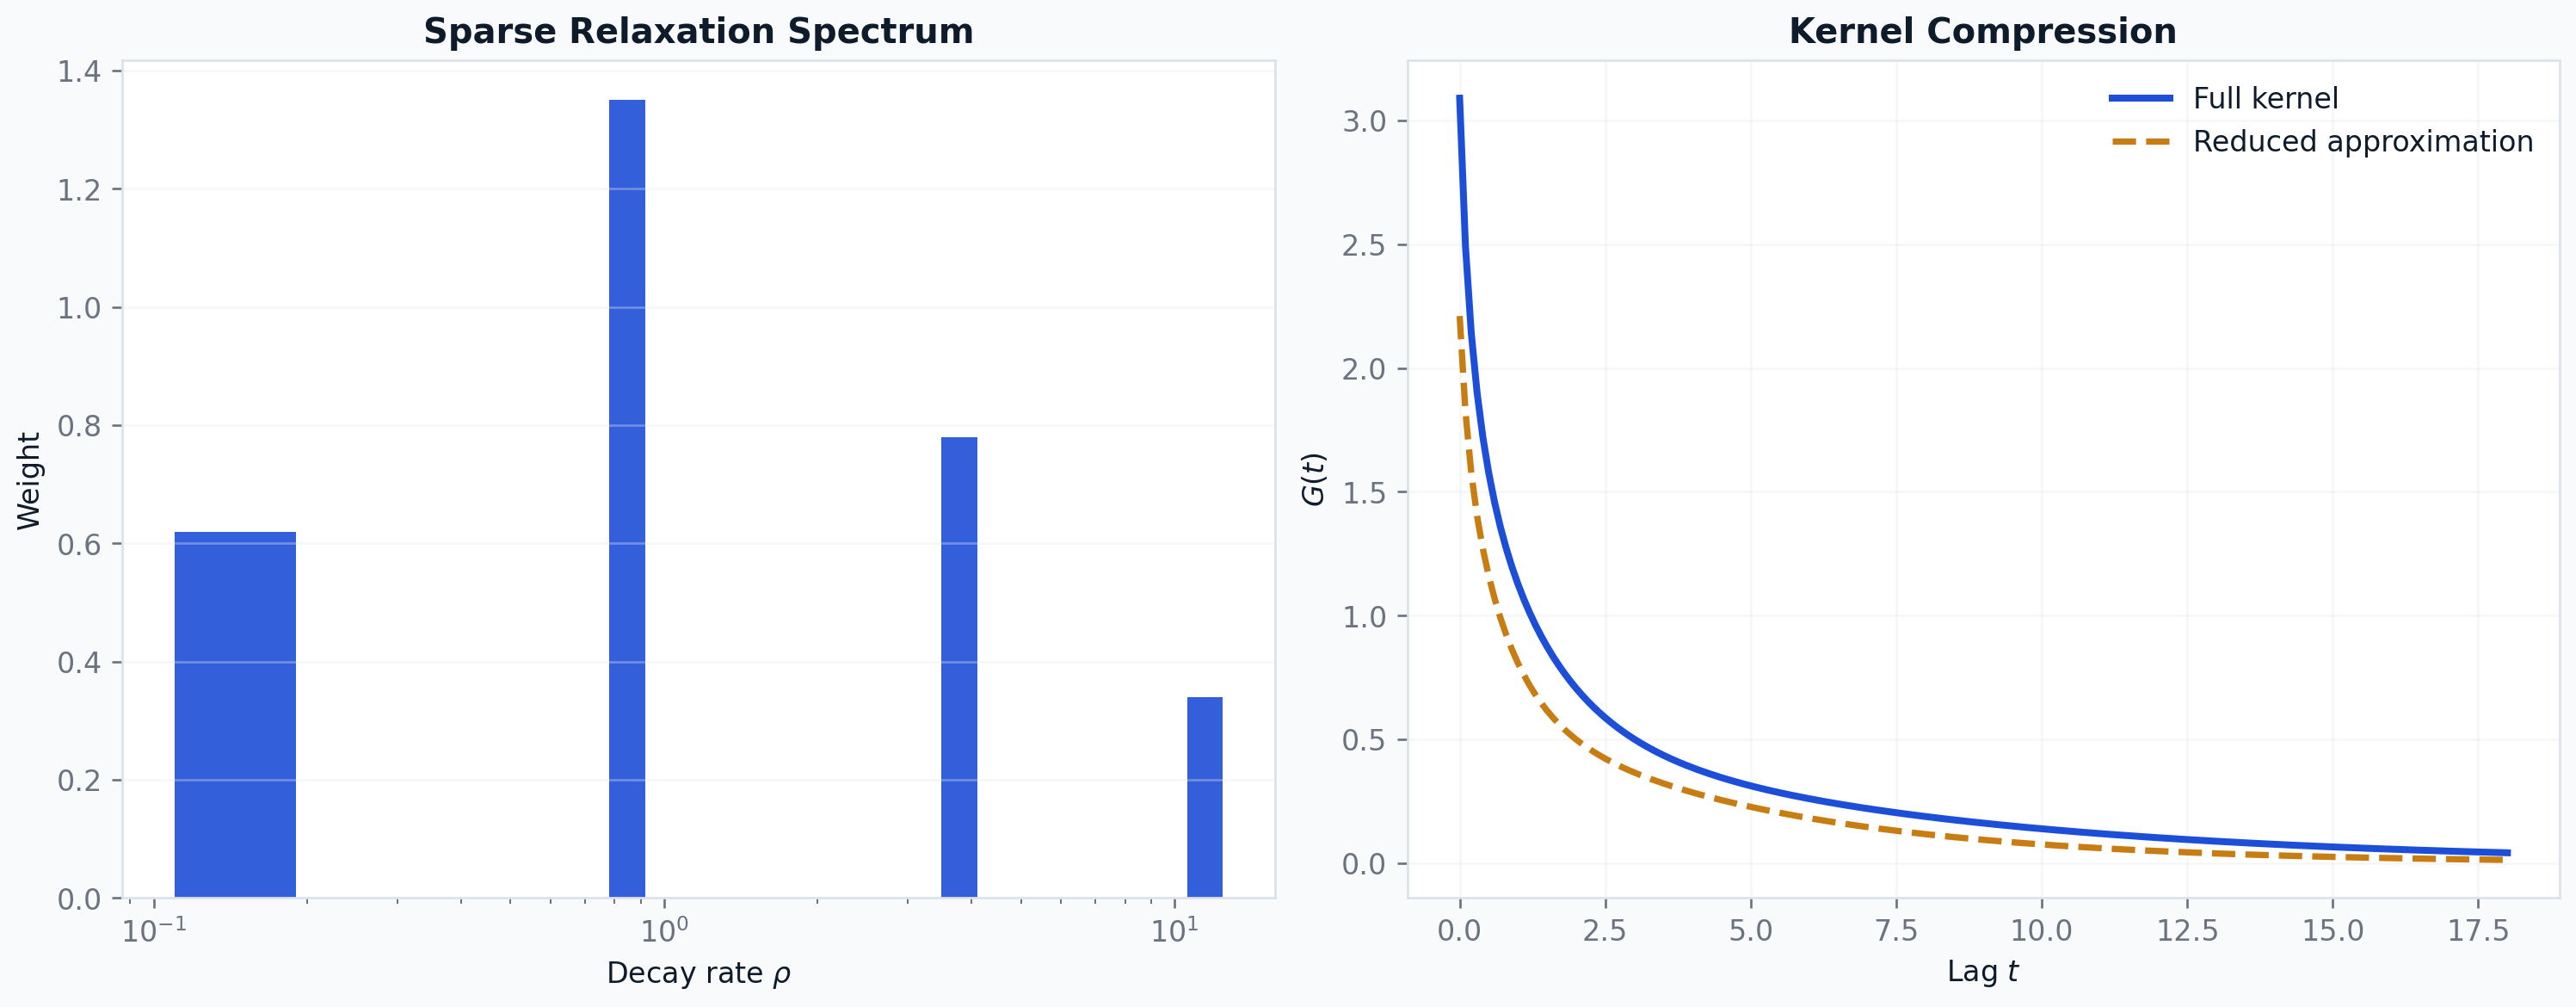
\includegraphics[width=\textwidth]{figures/generated/relaxation_spectrum.png}
\caption{Stylized reconstruction view. The left panel shows a sparse relaxation spectrum, while the right panel compares the full transient kernel (blue) with a sparse reduced approximation (dashed gold).}
\label{fig:relaxation-spectrum}
\end{figure}

\section{Implementation Notes}
\REV
The implementation details are standard and we keep them brief. Microstructure noise is handled with pre-averaging using the Bartlett kernel in the sense of Jacod et al.~\cite{JacodEtAl2009}, and the same pre-averaged returns feed the smoothed periodograms. Jumps are filtered by thresholding in the spirit of Mancini~\cite{Mancini2009}. Multi-asset extensions use Hayashi--Yoshida-style covariance correction under asynchrony, while slowly varying regimes are handled through rolling-window estimation rather than through a separate long-memory asymptotic theory. Long-memory order flow itself is outside the scope of the present paper.

\section{Monte Carlo Evidence}\label{sec:monte-carlo}

\subsection{Design}
We validate the test in a stylized spectral Monte Carlo under the two-mode kernel
\[
  G(t)=1.2e^{-0.4t}+0.7e^{-2.2t},
\]
with thermal index $\Theta=0.35$. Under the null, spectra satisfy the FDT exactly. Under the alternative, we inflate the mid-frequency price spectrum by a localized stress factor while holding the impact kernel fixed, thereby generating a nonzero deviation profile. For each sample size $n\in\{2^{12},2^{14},2^{16}\}$ we use 500 Monte Carlo replications for size and power, and 1000 parametric-bootstrap replications to estimate the $5\%$ critical value under $H_0$.

\subsection{Size and Power}
The effective smoothing parameter $m$ denotes the number of frequencies in the local averaging window used to stabilize the spectral estimates.

\begin{table}[t]
\centering
\caption{Monte Carlo performance of the null-enforcing FDT test}
\begin{tabular}{ccccc}
\toprule
$n$ & Replications & Effective smoothing $m$ & Size (5\% nominal) & Power \\
\midrule
$2^{12}$ & 500 & 8  & $0.048\,(0.010)$ & $0.180\,(0.017)$ \\
$2^{14}$ & 500 & 16 & $0.060\,(0.011)$ & $0.358\,(0.021)$ \\
$2^{16}$ & 500 & 32 & $0.042\,(0.009)$ & $0.748\,(0.019)$ \\
\bottomrule
\end{tabular}
\vspace{0.4em}

\parbox{0.9\textwidth}{\footnotesize Parentheses report Monte Carlo standard
errors computed from 500 replications. Here $m$ is the number of frequencies in
the smoothing window (bandwidth). Size stays close to the nominal $5\%$ level,
while power rises with sample size as spectral smoothing improves.}
\label{tab:monte-carlo}
\end{table}

Figure~\ref{fig:monte-carlo-delta} shows one representative draw under the alternative at $n=2^{14}$. The estimated deviation functional tracks the sign and broad shape of the true mid-frequency stress profile, which helps explain the power gains reported in \cref{tab:monte-carlo}.

We also ran an auxiliary theorem-matched manipulation-signal check in which the nonequilibrium deformation is designed to generate a positive deviation band on $B=[0.22,0.90]$ and the neighboring Kramers--Kronig band is $B'=[1.08,1.26]$. Among rejecting draws in that auxiliary design, the numerically estimated neighboring-band negativity condition is satisfied in $87.6\%$, $98.0\%$, and $100\%$ of cases for $n=2^{12}$, $2^{14}$, and $2^{16}$ respectively. This does not replace the theorem, but it shows that the neighboring-band mechanism is numerically credible in the simulated data once the alternative is constructed to match the theorem's logic.

\begin{figure}[t]
\centering
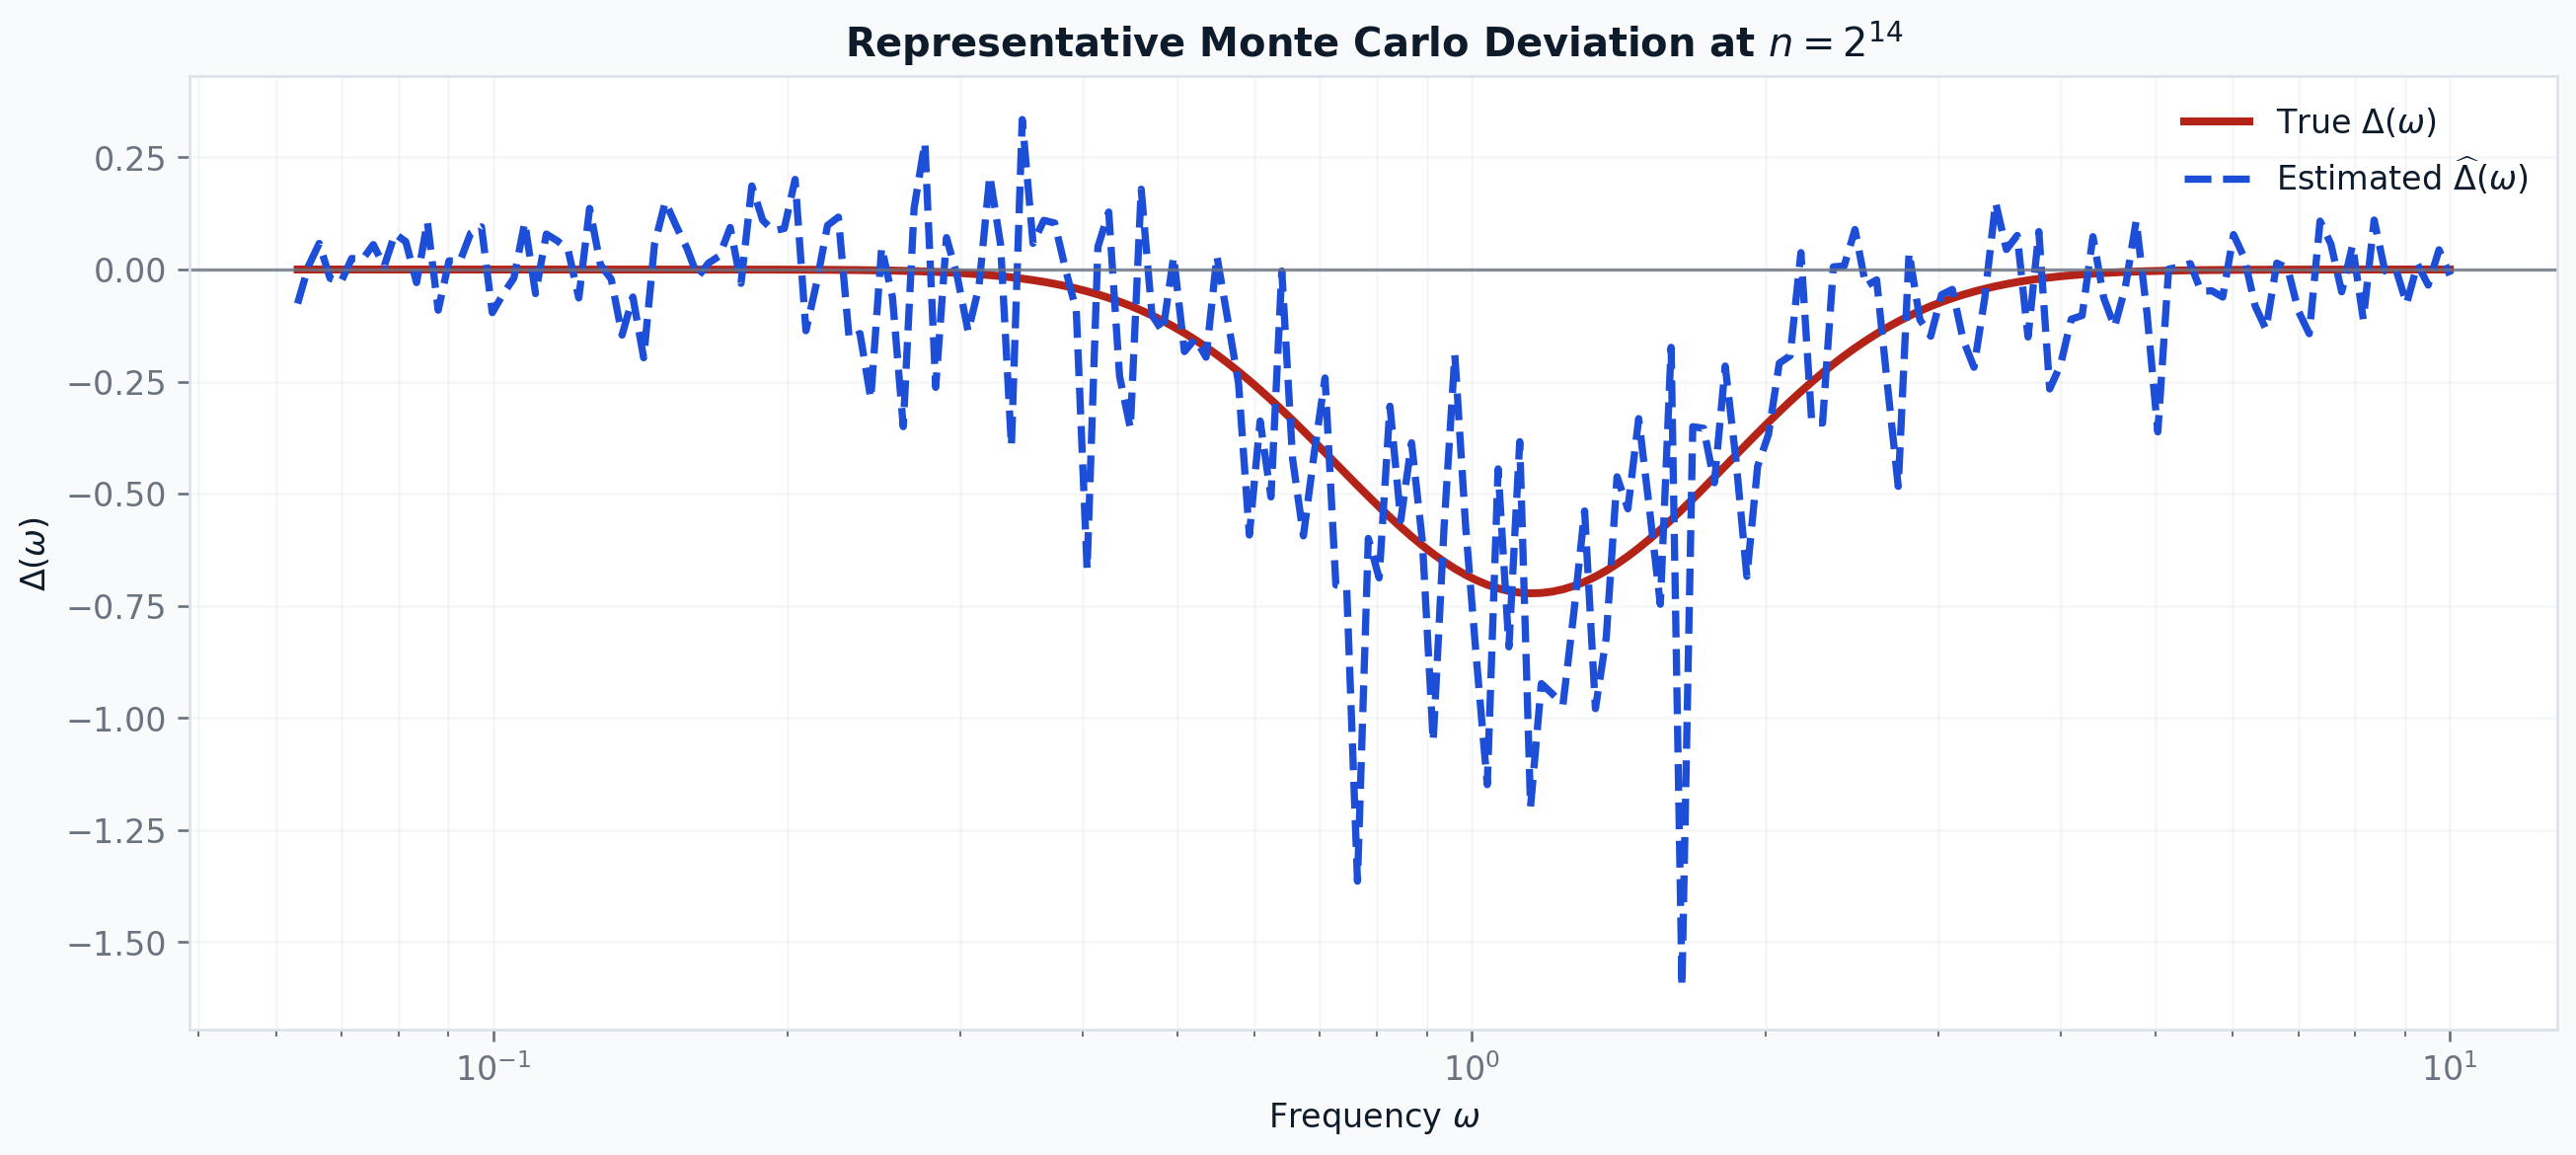
\includegraphics[width=0.88\textwidth]{figures/generated/monte_carlo_delta.png}
\caption{Representative simulation at $n=2^{14}$ under the two-mode kernel $G(t)=1.2e^{-0.4t}+0.7e^{-2.2t}$. The solid red line is the true $\Delta(\omega)$ and the dashed blue line is the estimated $\widehat{\Delta}(\omega)$. The estimate tracks the sign and shape of the true mid-frequency stress profile, but remains noisy at the lowest frequencies.}
\label{fig:monte-carlo-delta}
\end{figure}

\section{Rolling-Window Validation}\label{sec:rolling}

\subsection{Design}
Monte Carlo size and power establish that the test behaves correctly in repeated sampling, but they do not yet show how the procedure behaves over evolving market states. We therefore run a rolling-window validation exercise in which we simulate $60$ consecutive sessions of length $n=2^{14}$ with the same two-mode kernel used in the Monte Carlo study, keep the bootstrap critical value fixed at its null-calibrated level, and let the spectrum move through three regimes:
\begin{enumerate}[label=\arabic*.]
  \item Sessions $1$--$20$: equilibrium benchmark.
  \item Sessions $21$--$40$: transition regime with a gradually emerging mid-frequency stress wedge.
  \item Sessions $41$--$60$: stressed regime with a large and persistent spectral distortion.
\end{enumerate}
For each session we compute the rolling estimate $\widehat{\Theta}$, the test statistic $\cT_n$, and the full curve $\widehat{\Delta}(\omega)$ on a dense frequency grid. This exercise remains synthetic rather than TAQ-based, but it clarifies how the diagnostic reacts to changing regimes before moving to real order-book data.

\subsection{Validation Readout}
\begin{table}[t]
\centering
\caption{Rolling-window validation across synthetic operating regimes}
\begin{tabular}{lcccc}
\toprule
Regime & Sessions & Rejection rate & Average $\widehat{\Theta}$ & Average peak $|\widehat{\Delta}|$ \\
\midrule
Equilibrium & 20 & 0.00 & 0.34086 & 0.32776 \\
Transition  & 20 & 0.10 & 0.38168 & 0.54619 \\
Stress      & 20 & 0.65 & 0.65307 & 2.73138 \\
\bottomrule
\end{tabular}
\vspace{0.4em}

\parbox{0.92\textwidth}{\footnotesize The rolling-window validation uses the same null-enforcing bootstrap as the main test. The stressed regime simultaneously raises the rejection rate, the inferred thermal index, and the magnitude of the deviation functional, producing a coherent operational readout rather than an isolated scalar alarm.}
\label{tab:rolling-validation}
\end{table}

Table~\ref{tab:rolling-validation} shows the central pattern. Equilibrium windows remain quiet, transition windows begin to drift, and stressed windows trigger rejection in nearly two-thirds of sessions. That is exactly the type of separation an applied reader wants to see before investing in a full TAQ deployment.

\begin{figure}[t]
\centering
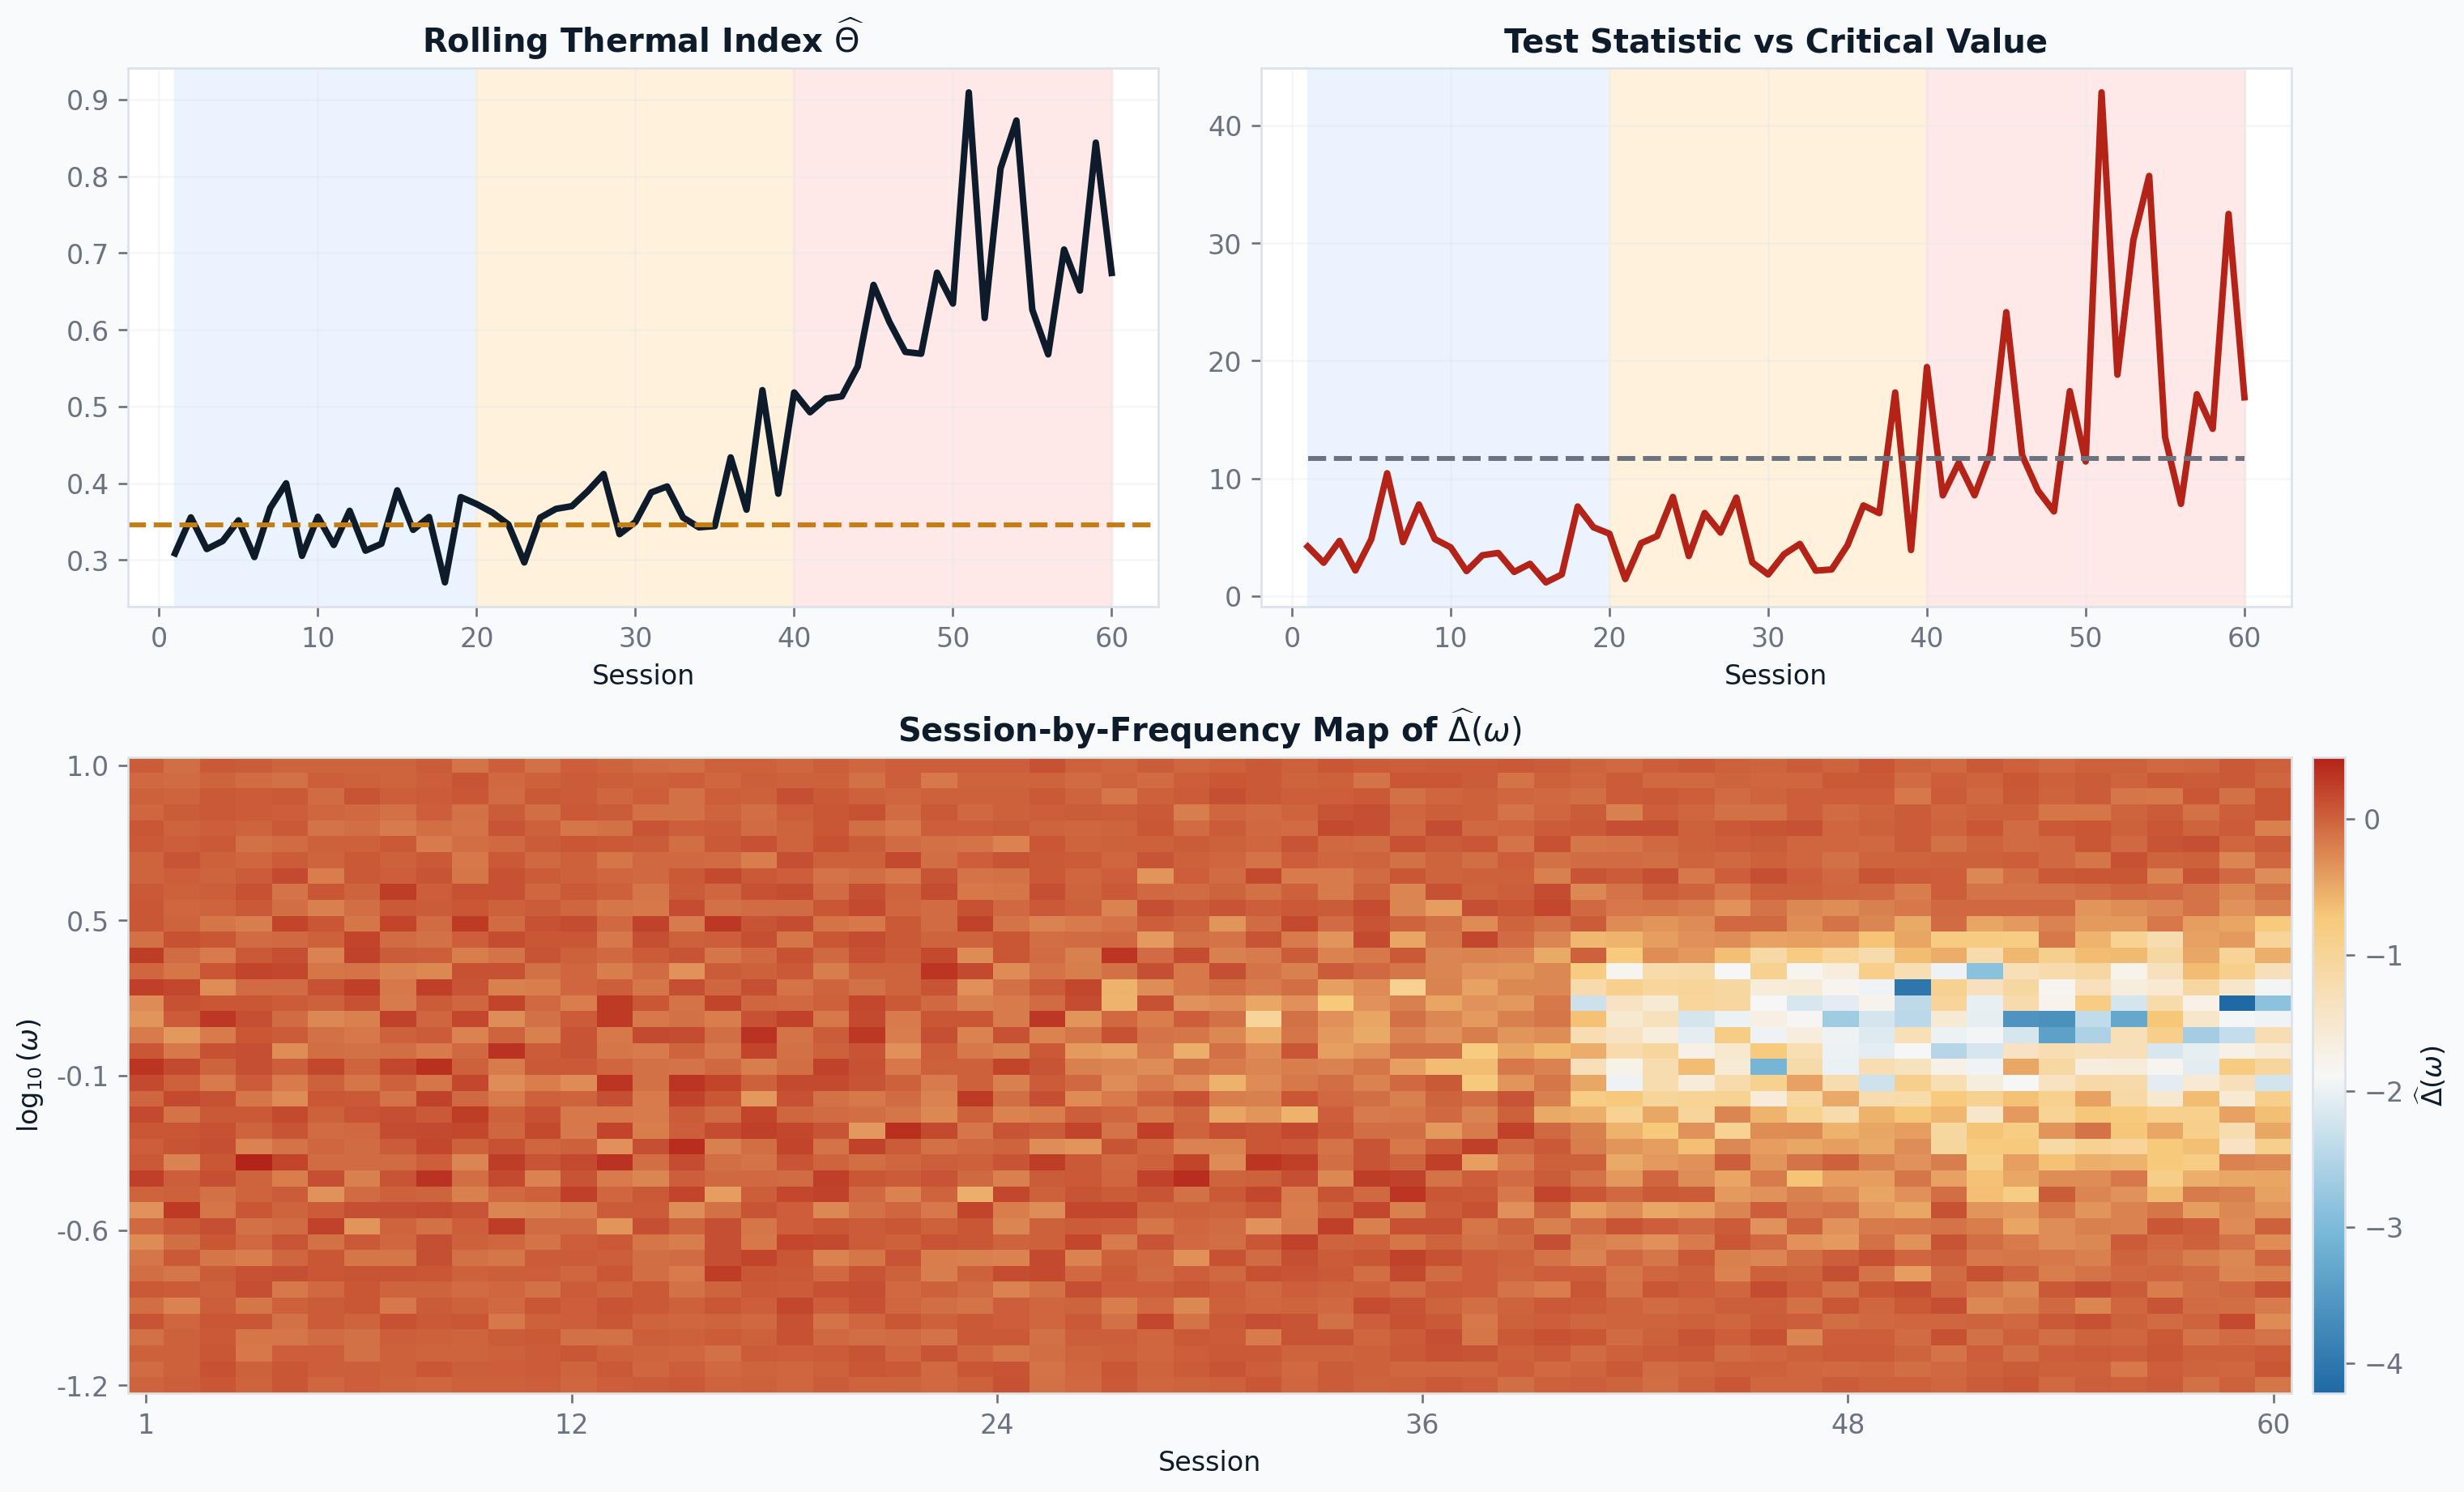
\includegraphics[width=\textwidth]{figures/generated/operational_validation.png}
\caption{Rolling-window validation panel. Top left: the estimated thermal index $\widehat{\Theta}$ across $60$ sessions, with regime shading. Top right: the session-level test statistic $\mathcal{T}_n$ against the fixed bootstrap critical value. Bottom: the corresponding session-by-frequency map of $\widehat{\Delta}(\omega)$, showing stress first concentrating in a mid-frequency band and then spreading as the stressed regime intensifies.}
\label{fig:operational-validation}
\end{figure}

\section{Real-Data LOBSTER Evidence}\label{sec:lobster-pilot}

\subsection{Data and Construction}
To demonstrate that the pipeline can be executed on genuine stock-market data, we use public LOBSTER samples for June 21, 2012. The main single-name illustration is AAPL, and we also run the same protocol on same-date samples for GOOG and AMZN to obtain a minimal liquid-stock cross-section under a common market environment. The samples contain the full NASDAQ message stream and the synchronized top-of-book state over the continuous trading day from 9:30 to 16:00. We aggregate the data to one-minute bins. Midquote returns are computed from the last best bid and best ask observed in each bin, and signed order flow is computed from executed volume only, using LOBSTER event types 4 and 5 with the exchange-provided trade direction. This is not yet a multi-week TAQ panel, but it is genuine trade-and-quote style market data with true trade direction rather than a price-based proxy.

\begin{remark}[Scope of the real-data evidence]
The real-data exercise is intentionally narrow rather than broad. Its purpose is to show that the estimation and testing pipeline can be executed on genuine order-book data and can produce economically interpretable intraday regime differences. The same-date GOOG and AMZN comparison names help guard against a pure one-name anecdote, but the exercise is not intended to support market-wide claims.
\end{remark}

\subsection{AAPL Windowed Evidence}
\REV
We split the day into three economically interpretable windows: the open (9:30--11:00), midday (11:30--14:30), and the close (14:30--16:00). In each window we estimate $\widehat{G}$ from the return-flow cross-spectrum, infer $\widehat{\Theta}$ from the frequency band where $\ImPart\widehat{G}>0$, and calibrate the null by the same null-enforcing bootstrap used in the main testing section. The empirical implementation uses the local ridge rule
\[
  \eta_n(\omega_j)=0.01\,\widehat S_Q(\omega_j),
\]
which is the exact rule implemented in the empirical script on the retained band.\footnote{\REV In the empirical implementation, replacing $\eta_n$ by $0.5\eta_n$ or $2\eta_n$ leaves the open/midday/close reject-vs.-nonreject classification unchanged and leaves the reported thermal-index and deviation-ratio patterns unchanged to the displayed precision. The ridge therefore stabilizes inversion without driving the substantive conclusions.}

\begin{table}[t]
\centering
\caption{AAPL LOBSTER evidence on June 21, 2012 (one-minute bins)}
\begin{tabular}{lcccc}
\toprule
Window & $\widehat{\Theta}$ & Deviation ratio & Bootstrap $p$-value & Reject at $5\%$ \\
\midrule
Open   & 4.074 & 0.216 & 1.000 & No \\
Midday & 1.167 & 1.104 & 0.003 & Yes \\
Close  & 2.225 & 0.686 & 0.358 & No \\
\bottomrule
\end{tabular}
\vspace{0.4em}

\parbox{0.92\textwidth}{\footnotesize The deviation ratio is $\|\widehat{\Delta}\|_{L^2}/\|\ImPart\widehat{G}\|_{L^2}$ over the retained frequency band. The result is intentionally local rather than universal: on this day the opening and closing windows are broadly consistent with the FDT, while the midday block shows a clear break.}
\label{tab:lobster-pilot}
\end{table}

The central empirical point is not that the FDT always holds or always fails. It is that the diagnostic separates regimes inside a single real trading day. On this AAPL sample, the opening and closing windows produce low deviation ratios and no rejection, whereas the midday block yields a sharp break with bootstrap $p=0.003$. Figure~\ref{fig:lobster-empirical} shows the same story visually: the normalized dissipation curve and normalized FDT benchmark lie close together in the opening and closing windows, but visibly separate at midday. The lower panel tracks the rolling thermal index across the day and marks the windows where the test rejects.

\begin{figure}[t]
\centering
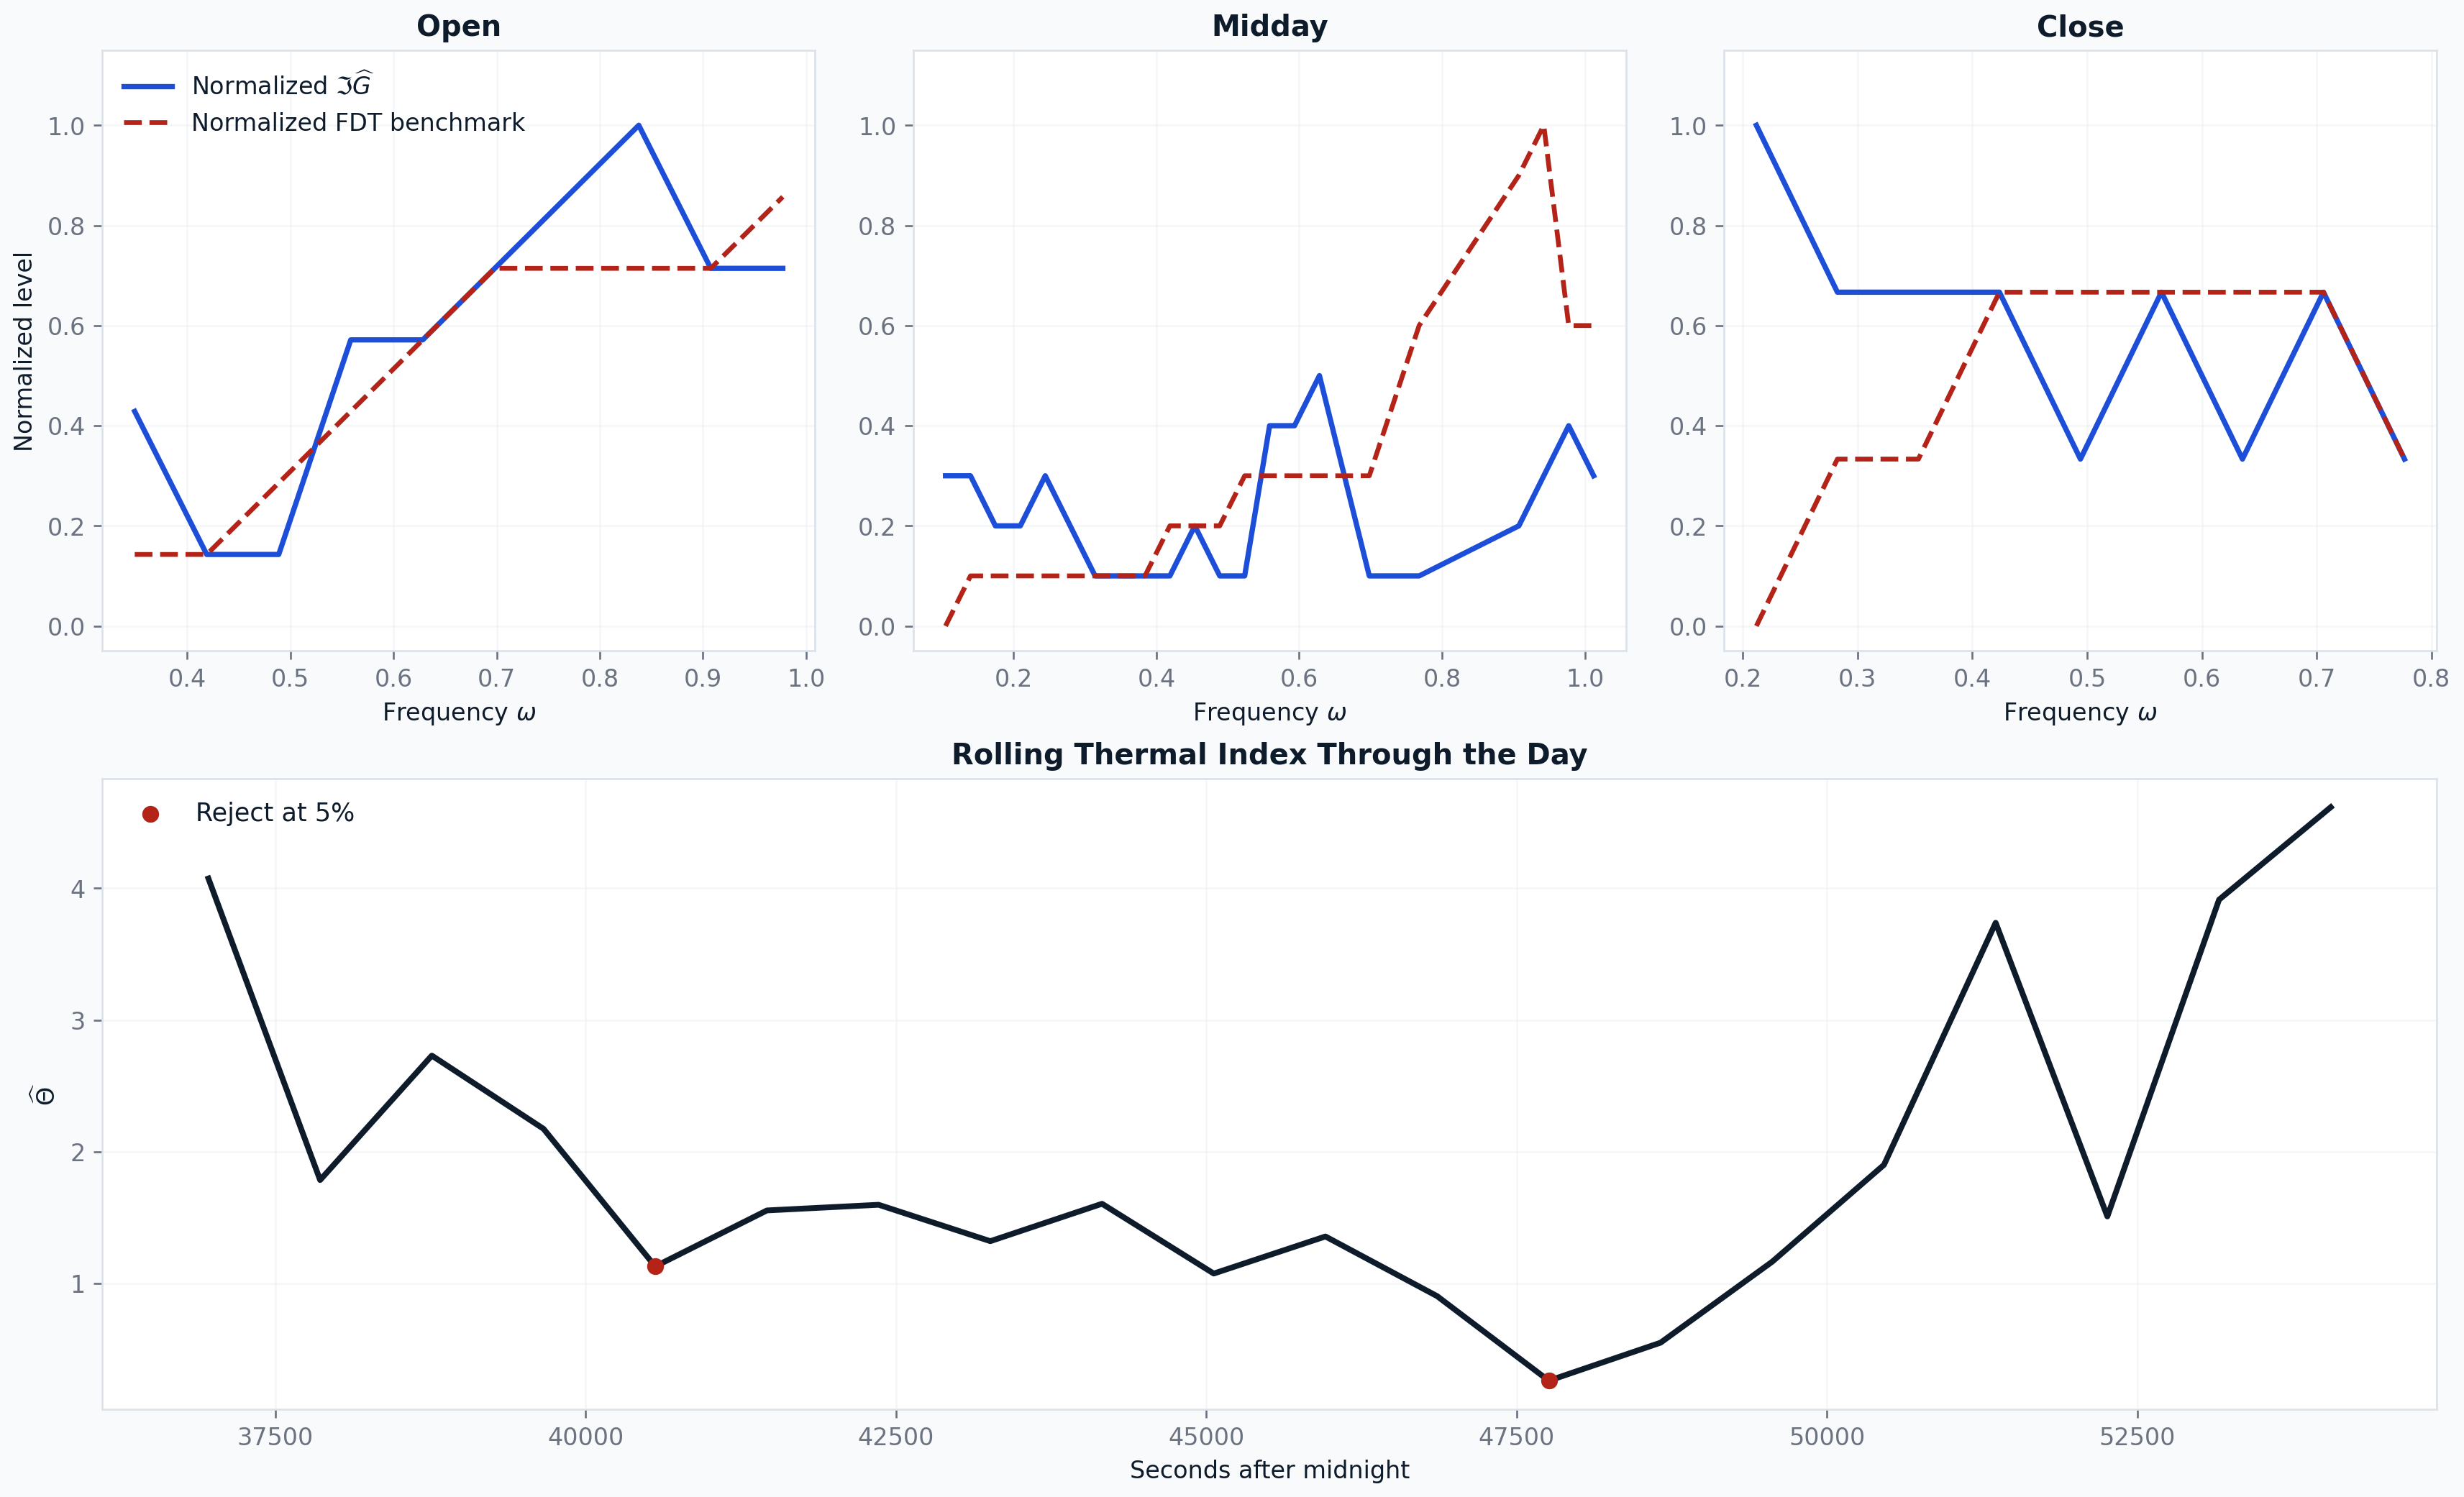
\includegraphics[width=\textwidth]{figures/generated/lobster_empirical.png}
\caption{AAPL LOBSTER evidence. Top row: normalized $\ImPart\Ghat(i\omega)$ (blue) against the normalized FDT benchmark $(\omega/(2\widehat{\Theta}))\widehat{S}_P(\omega)$ (dashed red) for the open, midday, and close windows. Bottom row: the rolling estimate of the thermal index $\widehat{\Theta}$ over the day; red markers identify rolling windows where the bootstrap test rejects at the $5\%$ level. The figure highlights an important distinction: $\widehat{\Theta}$ is a market-state variable, whereas $\widehat{\Delta}$ is the equilibrium-breakdown diagnostic.}
\label{fig:lobster-empirical}
\end{figure}

\subsection{Interpretation}
The LOBSTER evidence suggests two empirical lessons. First, the proposed FDT diagnostic is not vacuous: it can survive contact with real order-book data without rejecting everywhere. Second, the thermal index and the deviation functional play different roles. In AAPL, the open has the largest estimated $\widehat{\Theta}$ but does not reject, which is consistent with an active but internally coherent market. Midday has a smaller $\widehat{\Theta}$ yet a much larger deviation ratio, indicating that ``temperature'' and ``distance from equilibrium'' should not be conflated. The current evidence is narrow rather than broad, but even this same-date cross-section shows why the two objects should be estimated jointly.

\subsection{Same-Date Cross-Section}
To check whether the AAPL intraday pattern is purely idiosyncratic, we run the
same open/midday/close protocol on public same-date LOBSTER samples for GOOG
and AMZN. Table~\ref{tab:lobster-cross-section} summarizes the resulting
diagnostics.

\begin{table}[t]
\centering
\caption{Same-date LOBSTER cross-section on June 21, 2012 (one-minute bins)}
\begin{tabular}{llccc}
\toprule
Symbol & Window & $\widehat{\Theta}$ & Deviation ratio & Reject at $5\%$ \\
\midrule
AAPL & Open   & 4.074 & 0.216 & No \\
AAPL & Midday & 1.167 & 1.104 & Yes \\
AAPL & Close  & 2.225 & 0.686 & No \\
GOOG & Open   & 0.217 & 0.294 & No \\
GOOG & Midday & 0.452 & 0.557 & No \\
GOOG & Close  & 1.798 & 0.583 & No \\
AMZN & Open   & 3.830 & 0.322 & No \\
AMZN & Midday & 2.675 & 0.612 & No \\
AMZN & Close  & 0.815 & 0.519 & No \\
\bottomrule
\end{tabular}
\vspace{0.4em}

\parbox{0.94\textwidth}{\footnotesize The same-date cross-section uses the same one-minute binning, transfer-function estimator, and null-enforcing bootstrap as the AAPL analysis. The main pattern is that a pronounced midday rejection appears in AAPL but does not mechanically appear in the other two public samples, which argues against interpreting the diagnostic as a trivial intraday seasonality effect.}
\label{tab:lobster-cross-section}
\end{table}

The cross-section changes the empirical reading of the results in an important way. The AAPL midday rejection is no longer just a one-name anecdote inside one day; it now stands against two same-date comparison names that do not reject in any of the three windows. GOOG is especially informative: its thermal index rises from the open into midday, yet the deviation ratio remains moderate and the null is not rejected, which points to a more active but still coherent liquidity state rather than a powerless test in a thin name. AMZN shows the same broader pattern of thermal variation without a corresponding equilibrium break. This remains narrower than panel evidence, but it is materially stronger than a single-series illustration.

\begin{figure}[t]
\centering
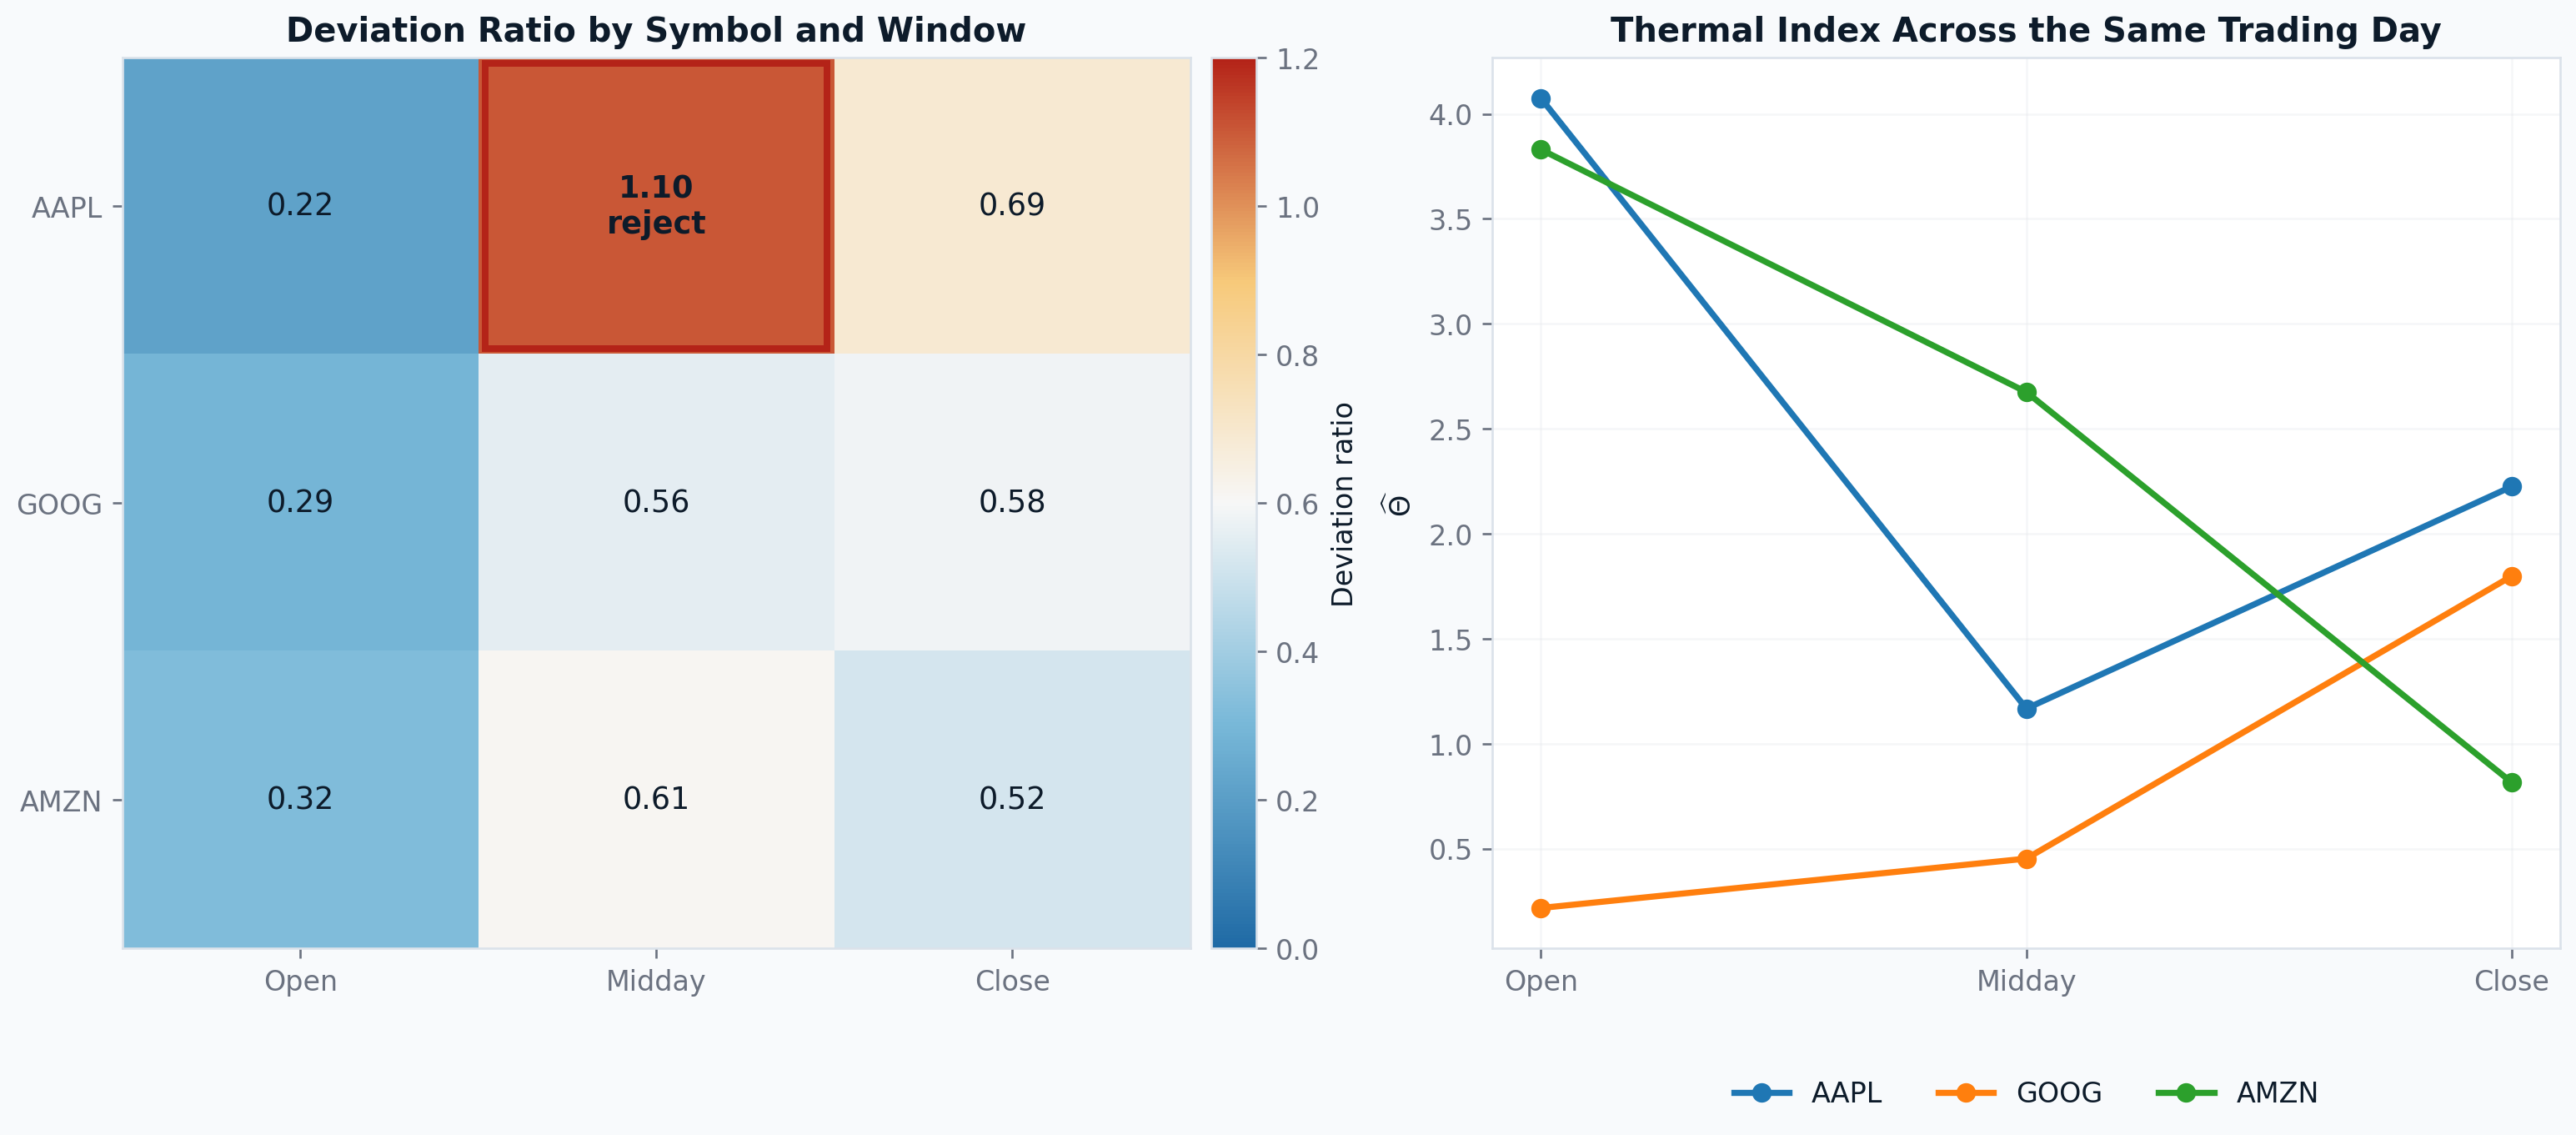
\includegraphics[width=\textwidth]{figures/generated/realdata_breakdown.png}
\caption{Real-data same-date cross-section. Left: deviation ratios for AAPL, GOOG, and AMZN across the open, midday, and close windows, with the rejecting cell outlined in red. Right: the corresponding thermal-index paths. The key empirical fact is compact: only AAPL exhibits a large midday breakdown signal, while GOOG and AMZN show thermal variation without rejection.}
\label{fig:realdata-breakdown}
\end{figure}

Figure~\ref{fig:realdata-breakdown} is the sharpest real-data finding in the paper. Out of the nine symbol-window cells in this public same-date study, only AAPL midday rejects. That is not a full panel study, but it is already stronger than a single-name illustration because it shows that the diagnostic is not merely echoing the common intraday shape of liquidity.

\subsection{A Market-State Map}
The most compact way to summarize the empirical program is to treat $\widehat{\Theta}$ and the deviation magnitude as two separate coordinates. Figure~\ref{fig:market-state-map} places the synthetic equilibrium, transition, and stress regimes alongside the real AAPL windows in the same plane. The resulting picture is useful because it turns an abstract identity into a state map: low-deviation points sit near equilibrium regardless of whether the market is ``cold'' or ``hot,'' while large-deviation points move into a breakdown region. This is where the paper has its clearest empirical payoff.

\begin{figure}[t]
\centering
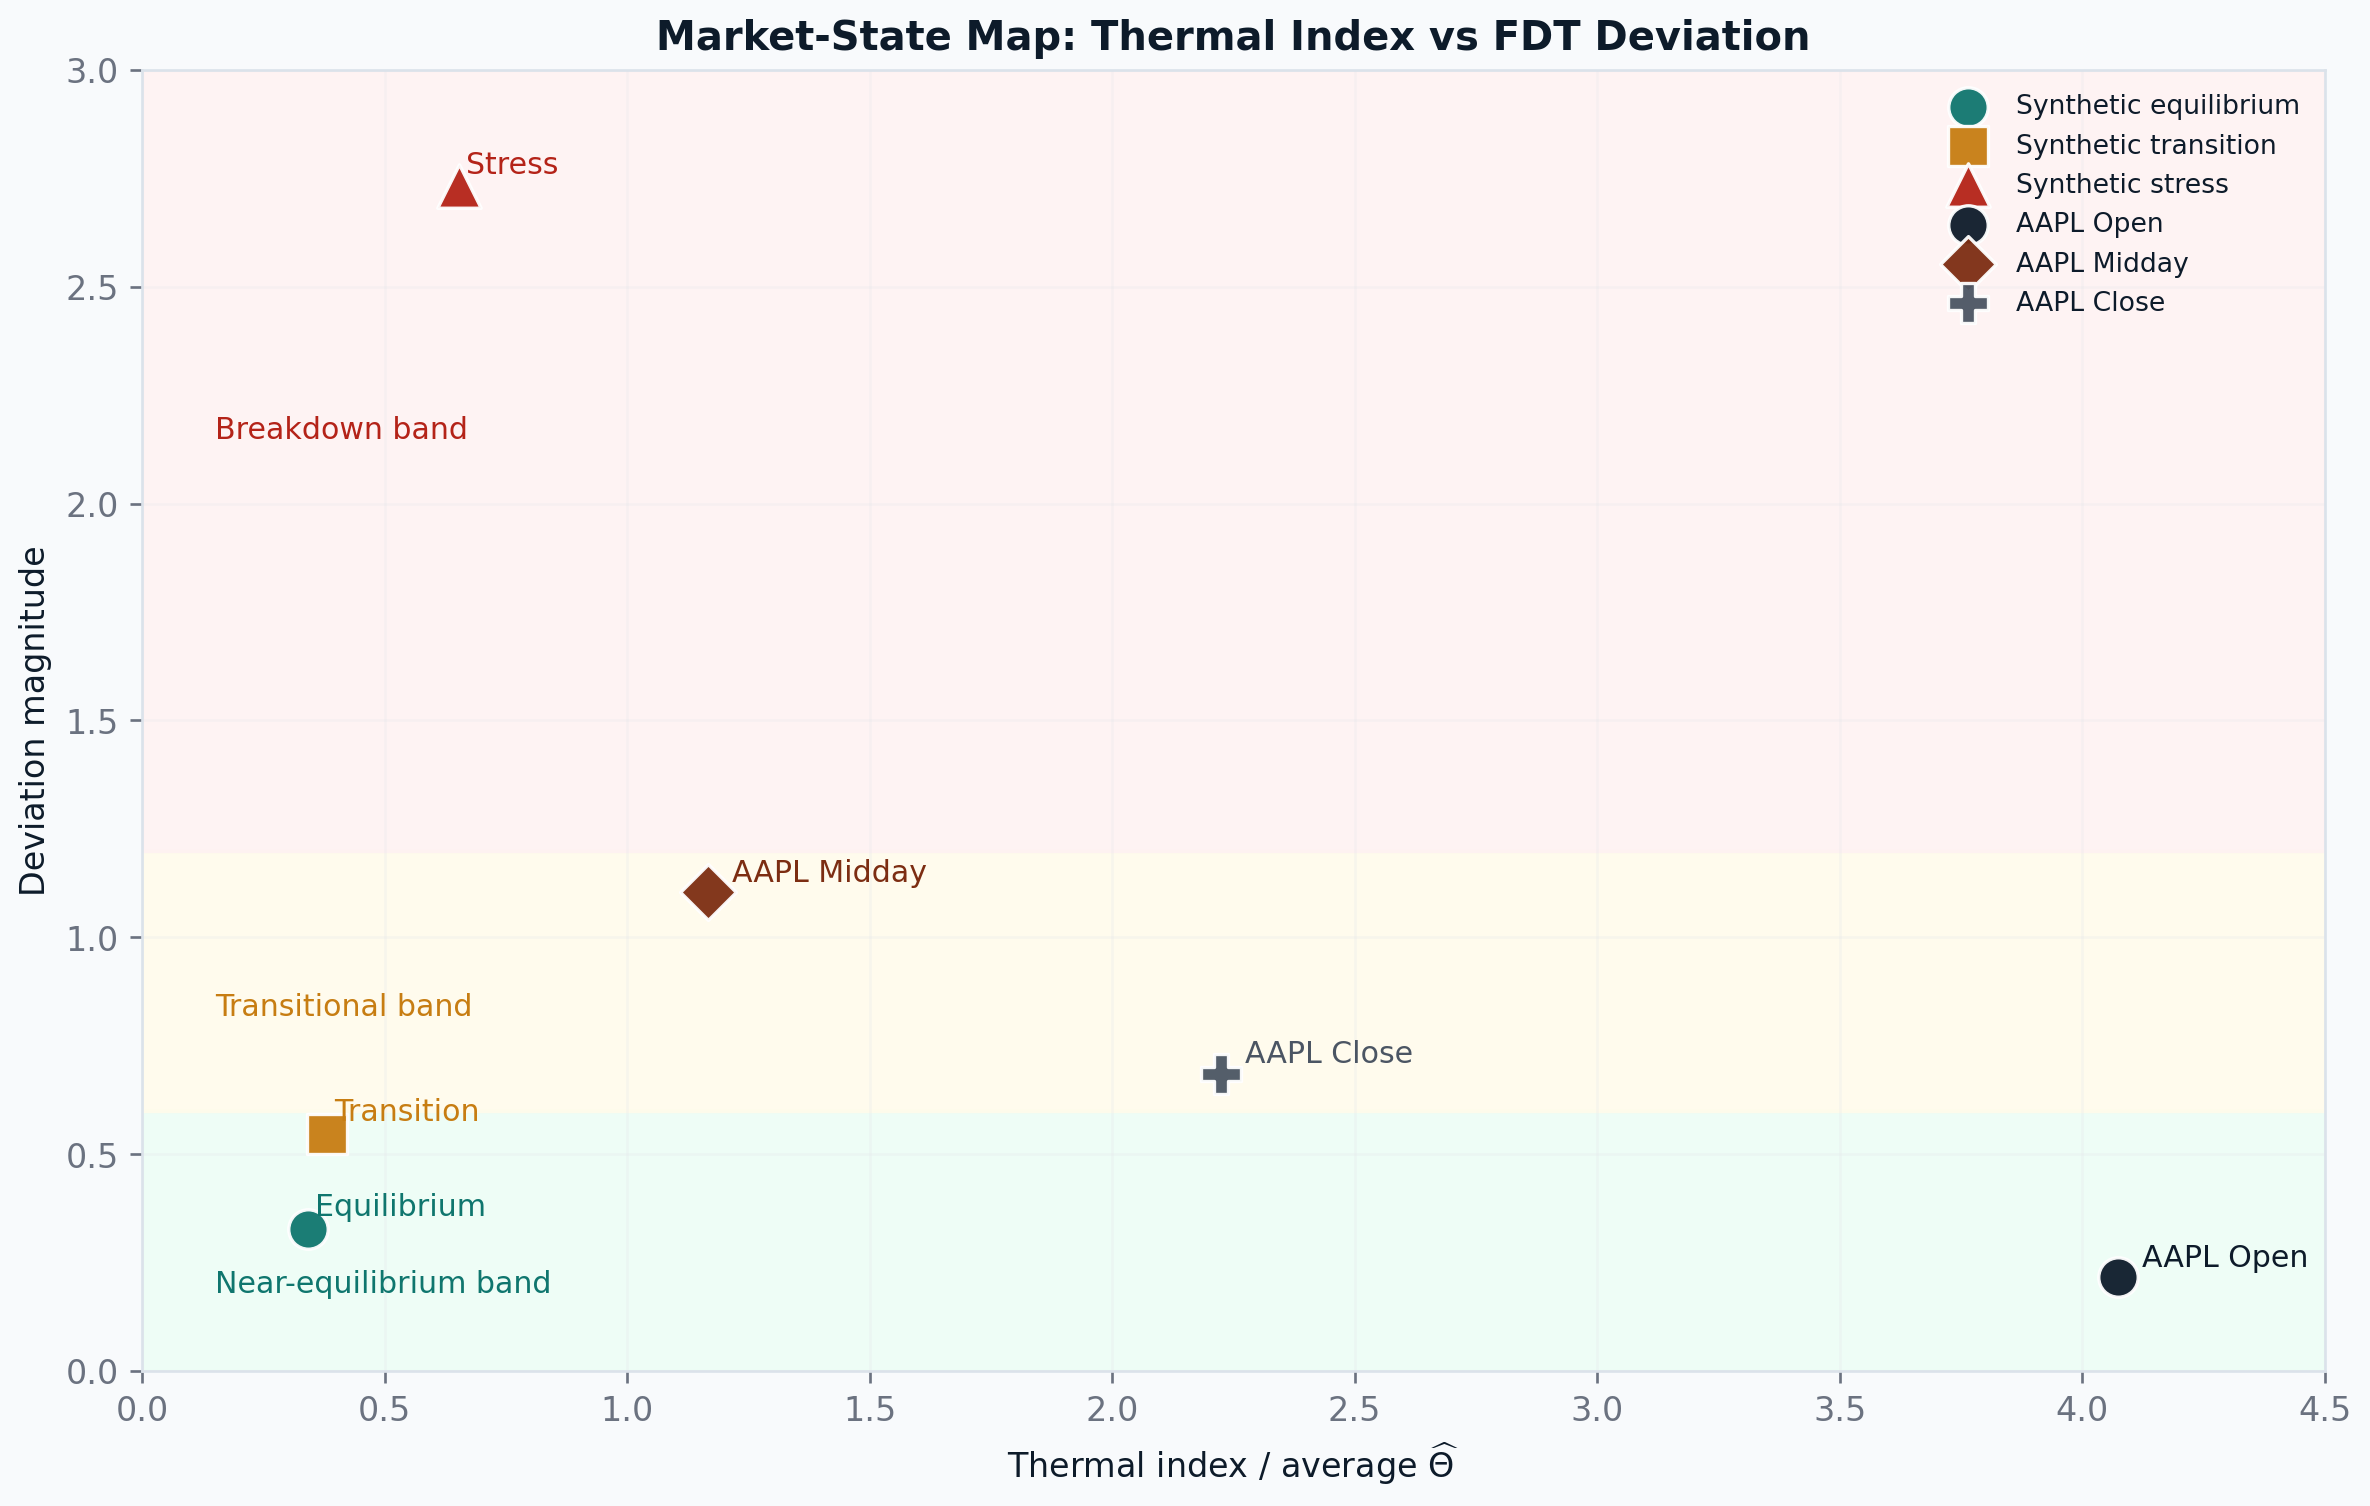
\includegraphics[width=0.82\textwidth]{figures/generated/market_state_map.png}
\caption{Market-state map. The horizontal axis is the thermal index and the vertical axis is a deviation magnitude: average peak $|\widehat{\Delta}|$ for the synthetic validation regimes and $\|\widehat{\Delta}\|_{L^2}/\|\ImPart \widehat{G}\|_{L^2}$ for the AAPL windows. Synthetic equilibrium, transition, and stress regimes occupy clearly separated zones, while the AAPL open, midday, and close windows land in empirically interpretable regions of the same map. The visual message is simple: temperature and equilibrium breakdown are distinct coordinates.}
\label{fig:market-state-map}
\end{figure}

\section{Interpretation and Next Empirical Step}\label{sec:roadmap}

\subsection{What rejection means}
\REV
The paper should be read as a falsification framework for a structured equilibrium class. If the FDT restriction fails on a frequency band of positive measure, then the observed market is not well described by the latent modal equilibrium model on that band. That is the main empirical content. The market-state map is useful because it separates two questions that are often conflated in practice: how active the market is, as summarized by $\widehat{\Theta}$, and how far the market is from the conditional equilibrium restriction, as summarized by $\widehat{\Delta}$.

\subsection{Current empirical limits}
\REV
The real-data evidence in this paper should be read as a focused order-book study, not as a market-wide validation exercise. The current cross-section is same-date and small by construction, so its role is to show that the diagnostic can isolate a concrete breakdown cell in genuine message data while avoiding blanket rejection elsewhere. Broader panel claims are therefore not inferred from this sample.

\subsection{Next empirical step}
\REV
The cleanest next empirical test is an event study around scheduled macro announcements. The model makes a sharp prediction: the deviation ratio should spike in the announcement window and then mean-revert, while $\widehat{\Theta}$ captures the surrounding liquidity regime. That design is more informative than simply adding more intraday plots because it asks the framework to succeed or fail against an externally timed stress event.

\subsection{Data and Code Availability}
Simulation code, plotting scripts, and the real-data analysis scripts used for the reported figures are collected in the public replication repository at \url{https://github.com/Atharva12081/fdt-market-impact}. The current real-data study is based on public LOBSTER samples for AAPL, GOOG, and AMZN on June 21, 2012. Replication files for any proprietary TAQ extension can be shared only subject to vendor licensing constraints. The author thanks colleagues and seminar participants for helpful discussions. No external funding was received, and the author declares no competing interests. Additional robustness checks and extended tables are described in the online supplement.

\section{Conclusion}
\REV
This study develops a conditional fluctuation--dissipation framework for transient market impact that is both structurally coherent and empirically testable. On the theory side, it analyzes the consequences of an explicit latent modal equilibrium model, links the resulting identity to passivity and no manipulation, and gives a linear-Gaussian foundation for the modal scaling. The converse theorem should be read in that same conditional spirit: it is a second-order-law characterization of the latent modal class, not a strategic derivation of equilibrium from unrestricted primitives. On the statistical side, the paper provides a concrete test, a structured inverse problem, controlled Monte Carlo evidence, and real-data LOBSTER evidence showing that the diagnostic can hold, fail, and recover within a single trading date across multiple names. The strongest payoff is empirical rather than axiomatic: once the thermal index and deviation functional are estimated jointly, they organize both synthetic and real observations into a coherent market-state map. In the data studied here, that map isolates one clear breakdown cell, AAPL at midday, while the same-date GOOG and AMZN windows remain non-rejecting.

\appendix

\section{Empirical Construction Details}
\REV
The LOBSTER study uses message-file event types $4$ and $5$ only, corresponding respectively to visible and hidden executions. The trading day is partitioned into consecutive one-minute bins on $[9{:}30,16{:}00)$, and each message is assigned to the unique bin containing its exchange timestamp. The midquote in a bin is the last observed top-of-book midpoint in that bin, namely $(\text{best ask}+\text{best bid})/2$, with carry-forward of the most recent midpoint if no new quote arrives before the bin closes. Signed order flow is the sum of executed shares in the bin with the sign taken directly from the LOBSTER trade-direction field in the message file, so buyer-initiated trades enter with sign $+1$ and seller-initiated trades with sign $-1$. Returns are one-minute log differences of the carried-forward midquote sequence. The ridge-regularized transfer estimator uses the local rule $\eta_n(\omega_j)=0.01\,\widehat S_Q(\omega_j)$ on the retained band.

\section{Selected References}
\begin{thebibliography}{99}

\bibitem{AbiJaberNeuman2025}
Abi Jaber, E. and Neuman, E. (2025).
\newblock Optimal liquidation with signals: the general propagator case.
\newblock \emph{Mathematical Finance}, 35(4), 841--866.

\bibitem{AitSahaliaJacod2014}
A{\"i}t-Sahalia, Y. and Jacod, J. (2014).
\newblock \emph{High-Frequency Financial Econometrics}.
\newblock Princeton University Press.

\bibitem{AlfonsiKlockSchied2016}
Alfonsi, A., Klock, F. and Schied, A. (2016).
\newblock Multivariate transient price impact and matrix-valued positive definite functions.
\newblock \emph{Mathematics of Operations Research}, 41(3), 914--934.

\bibitem{AndersonMoore1979}
Anderson, B.~D.~O. and Moore, J.~B. (1979).
\newblock \emph{Optimal Filtering}.
\newblock Prentice-Hall.

\bibitem{BaiPerron2003}
Bai, J. and Perron, P. (2003).
\newblock Computation and analysis of multiple structural change models.
\newblock \emph{Journal of Applied Econometrics}, 18(1), 1--22.

\bibitem{BouchaudFarmerLillo2009}
Bouchaud, J.-P., Farmer, J.~D. and Lillo, F. (2009).
\newblock How markets slowly digest changes in supply and demand.
\newblock In \emph{Handbook of Financial Markets: Dynamics and Evolution}, 57--160.

\bibitem{Brillinger2001}
Brillinger, D.~R. (2001).
\newblock \emph{Time Series: Data Analysis and Theory}.
\newblock SIAM Classics in Applied Mathematics.

\bibitem{Dahlhaus1997}
Dahlhaus, R. (1997).
\newblock Fitting time series models to nonstationary processes.
\newblock \emph{Annals of Statistics}, 25(1), 1--37.

\bibitem{Dahlhaus1996}
Dahlhaus, R. (1996).
\newblock On the Kullback--Leibler information divergence of locally stationary processes.
\newblock \emph{Stochastic Processes and their Applications}, 62(1), 139--168.

\bibitem{DelbaenSchachermayer1994}
Delbaen, F. and Schachermayer, W. (1994).
\newblock A general version of the fundamental theorem of asset pricing.
\newblock \emph{Mathematische Annalen}, 300, 463--520.

\bibitem{EnglHankeNeubauer1996}
Engl, H.~W., Hanke, M. and Neubauer, A. (1996).
\newblock \emph{Regularization of Inverse Problems}.
\newblock Kluwer.

\bibitem{Gatheral2010}
Gatheral, J. (2010).
\newblock No-dynamic-arbitrage and market impact.
\newblock \emph{Quantitative Finance}, 10(7), 749--759.

\bibitem{HayashiYoshida2005}
Hayashi, T. and Yoshida, N. (2005).
\newblock On covariance estimation of non-synchronously observed diffusion processes.
\newblock \emph{Bernoulli}, 11(2), 359--379.

\bibitem{HubermanStanzl2004}
Huberman, G. and Stanzl, W. (2004).
\newblock Price manipulation and quasi-arbitrage.
\newblock \emph{Econometrica}, 72(4), 1247--1275.

\bibitem{JacodProtter2012}
Jacod, J. and Protter, P. (2012).
\newblock \emph{Discretization of Processes}.
\newblock Springer.

\bibitem{JacodEtAl2009}
Jacod, J., Li, Y., Mykland, P.~A., Podolskij, M. and Vetter, M. (2009).
\newblock Microstructure noise in the continuous case: the pre-averaging approach.
\newblock \emph{Stochastic Processes and their Applications}, 119(7), 2249--2276.

\bibitem{Kyle1985}
Kyle, A.~S. (1985).
\newblock Continuous auctions and insider trading.
\newblock \emph{Econometrica}, 53(6), 1315--1335.

\bibitem{Mancini2009}
Mancini, C. (2009).
\newblock Non-parametric threshold estimation for models with stochastic diffusion coefficient and jumps.
\newblock \emph{Scandinavian Journal of Statistics}, 36(2), 270--296.

\bibitem{Natterer1984}
Natterer, F. (1984).
\newblock Error bounds for Tikhonov regularization in Hilbert scales.
\newblock \emph{Applicable Analysis}, 18(1--2), 29--37.

\bibitem{ObizhaevaWang2013}
Obizhaeva, A.~A. and Wang, J. (2013).
\newblock Optimal trading strategy and supply/demand dynamics.
\newblock \emph{Journal of Financial Markets}, 16(1), 1--32.

\bibitem{RosenbaumTomas2022}
Rosenbaum, M. and Tomas, M. (2022).
\newblock Admissibility of cross-impact models.
\newblock \emph{Frontiers of Mathematical Finance}, 1(4), 491--523.

\bibitem{TodorovTauchen2012}
Todorov, V. and Tauchen, G. (2012).
\newblock The realised Laplace transform of volatility.
\newblock \emph{Econometrica}, 80(3), 1105--1127.

\bibitem{Willems1972}
Willems, J.~C. (1972).
\newblock Dissipative dynamical systems, part I: general theory.
\newblock \emph{Archive for Rational Mechanics and Analysis}, 45(5), 321--351.

\end{thebibliography}

\end{document}
